% ----------------------------------------------------------------------------
% File: NaVisu4D.tex
% Usage:        Latex2e
% Creation :  25 juin 2020 sergemorvan29@gmail.com
% Revised:    24 décembre 2020 
% Revised:   
% ----------------------------------------------------------------------------
\documentclass[12pt, a4paper]{book}
% ----------------------------------------------------------------------------
%-------------------------------------------------------------------------
\usepackage{helvet}
\usepackage[utf8]{inputenc}
\usepackage[french]{babel}
\usepackage{moreverb}
\usepackage{eurosym}
\usepackage{index}
\usepackage{amsfonts}
\usepackage{graphics}
\usepackage{listings}
\usepackage{hyperref}
%\usepackage{html}
\usepackage{multimedia}
\usepackage{pgfpages}
\usepackage{pgf,xcolor,tikz}
\usepackage{rotating}
\usepackage{framed}
\usepackage[framed,hyperref,standard]{ntheorem}
\usepackage{fancyhdr,lastpage}
\usepackage{fancyvrb}

%-------------------------------------------------------------------------
% --- Commandes --------------------------------------------------------------
\renewcommand{\chaptermark}[1]{\markboth{#1}{}}

\renewcommand\contentsname{Table des mati\`eres}
\def\ladate{mars 2021}
\def\mot-cle#1{
	{\noindent {\bf Mots-cl\'es} : #1\vspace{-.5em}\vspace{0pt}}
	\def\mot-cle{\par}
}

\def\biblio#1{\subsection{R\'ef\'erences}\list
	{[\arabic{enumi}]}{\settowidth\labelwidth{[#1]}\leftmargin\labelwidth
		\advance\leftmargin\labelsep
		\usecounter{enumi}}
	\def\newblock{\hskip .11em plus .33em minus .07em}
	\sloppy\clubpenalty4000\widowpenalty4000
	\sfcode`\.=1000\relax}
\let\endbiblio=\endlist


% --- Identification du document ---------------------------------------------
\def\soustitre{\bf\sc Visualisation, simulation de données géoréférencées en 4D}
\def\projet{\bf\sc NaVisu4D}
\def\sousprojet{\bf\sc Dossier de utilisateur}
\def\titre{\bf\sc NaVisu4D }
\def\auteur{\sc{Serge}}
\def\leclient{Projet Open Source}
\def\lauteur{Lithops}
\def\leverif{l}
\def\chef{Serge}
\def\lechef{sm}
\def\laversion{0.2}
\def\sujet{\sc Manuel utilisateur } 

% --- Mise en page ------------------------------------------------------------
\setlength{\textwidth}{17.5cm}
\setlength{\textheight}{24.6cm}
\headsep=2cm
\footskip=1.5cm
\hoffset=-2cm
\voffset=-2.5cm
%--------------------------------------------------------------------------
% Changement de la syntaxe de la commande \chapter

\makeatletter 

%-------------------------------------------------------------------------
\hypersetup{
	bookmarks=true,         % show bookmarks bar?
	unicode=false,          % non-Latin characters in Acrobat’s bookmarks
	pdftoolbar=true,        % show Acrobats toolbar?
	pdfmenubar=true,        % show Acrobats menu?
	pdffitwindow=false,     % window fit to page when opened
	pdfstartview={FitH},    % fits the width of the page to the window
	pdftitle={My title},    % title
	pdfauthor={Lithops},     % author
	pdfsubject={NaVisu},   % subject of the document
	pdfcreator={Lithops},   % creator of the document
	pdfproducer={Producer}, % producer of the document
	pdfkeywords={keyword1} {key2} {key3}, % list of keywords
	pdfnewwindow=true,      % links in new window
	colorlinks=false,       % false: boxed links; true: colored links
	linkcolor=red,          % color of internal links
	citecolor=green,        % color of links to bibliography
	filecolor=magenta,      % color of file links
	urlcolor=cyan           % color of external links
}

%--------------------------------------------------------------------------
\pgfdeclareimage[width=2cm,interpolate=true]{navisuLogo}{images/Logotv2020}

\pagestyle{fancy}
\fancyhead[LE,LO]{\pgfuseimage{navisuLogo}}
\fancyhead[CE,CO]{\sc Visualisation, simulation de données géoréférencées en 4D }
\fancyhead[RE,RO]{2021 -- \thepage/\pageref{LastPage}}
\fancyfoot[LE,LO]{}
\fancyfoot[CE,CO]{\pgfuseimage{footline-enib-adresse}}
\fancyfoot[RE,RO]{}
\renewcommand{\headrulewidth}{0pt}
\renewcommand{\footrulewidth}{0pt}


%--------------------------------------------------------------------------
\cfoot{
\includegraphics[width=18.5cm]{images/bas-page.png}}
\rfoot{\raisebox{.3cm}{\textcolor{black}{\scriptsize{Version \laversion \ - 
				\ladate}}}}

%\SetWatermarkText{\sc Projet}
%\SetWatermarkScale{4}
\begin{document}
	% --- Commandes --------------------------------------------------------------
\newcommand{\nav}{{\sc NaVisu4D}\ }
\newcommand{\tv}{{\sc Terre Virtuelle \ }}

% ----------------------------------------------------------------------------
\begin{titlepage}
% ---------------
\begin{center}
{\LARGE\sc Association Terre Virtuelle}\\
\vspace{2cm}
\mbox{\LARGE \sc NaVisu4D}\\
\vspace{1cm}
\href{https://terrevirtuelle.org/Navisu4D}{http://terrevirtuelle.org/Navisu4D}

\vspace{1cm}
\mbox{\LARGE \sc Manuel utilisateur}\\
\vspace{0.5cm}

\mbox{\LARGE \sc Version 0.2 }\\
\vspace{0.5cm}

\begin{bfseries}

\begin{Huge}
\soustitre
\end{Huge}

\vspace{.8cm}

\null\vfill

%%%%%%%%%%%%%%%%%%%%%%%%%%%%%%%%%%%%%%%%%%%%%%%%%%%%%%%%%%%%%%%%%%%%%%

\begin{center}
	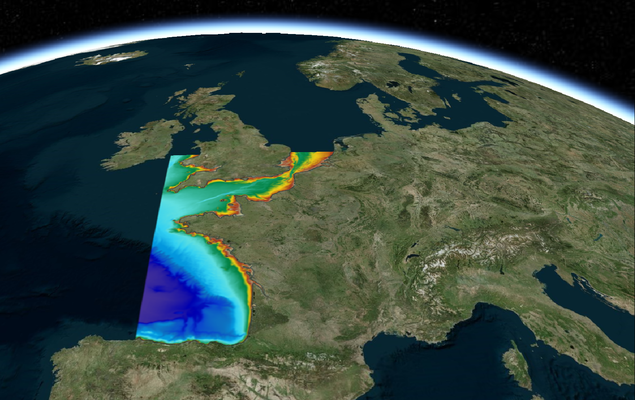
\includegraphics[width=16cm, height=10cm]{images/navisu4D_v2.png}
\end{center}

%%%%%%%%%%%%%%%%%%%%%%%%%%%%%%%%%%%%%%%%%%%%%%%%%%%%%%%%%%%%%%%%%%%%%%%
\null\vfill

\vspace{1cm}
2021

\end{bfseries}
\end{center}

\end{titlepage}

\hbox{}



%%%%%%%%%%%%%%%%%%%%%%%%%%%%%%%%%%%%%%%%%%%%%%%%%%%%%%%%%%%%%%%%%
\chapter{Le Projet NaVisu4D}
%%%%%%%%%%%%%%%%%%%%%%%%%%%%%%%%%%%%%%%%%%%%%%%%%%%%%%%%%%%%%%%%%
\section{Objet du document}
Ce document présente les différentes options, actuellement implémentées de 
\nav, le projet est encore à l'état de prototype, ces fonctionnalités sont susceptibles d'être modifiées, d'autres seront ajoutées. \\
Le site : \href{https://terrevirtuelle.org/Navisu4D}{https://terrevirtuelle.org/Navisu4D} est ouvert à l'utilisation.
\section{Objectifs du projet}
L'objectif du projet \nav est de représenter toutes données géoréférencées sur un globe terrestre virtuel en 3D. 
Ces données peuvent être cartographiques, provenant d'un service web : WMS, WMTS, WFS ou autres, elles peuvent aussi être des fichiers 3D comme des objets : navires, avions, bâtiments, des fichiers de données vectorielles : GeoJSON, ShapeFile, \ldots
Ainsi que des données de simulation temporelles.\\
Le logiciel \nav est une application web, nécessitant  un PC, tablette, téléphone, permettant l'affichage de la 3D et un navigateur moderne supportant WebGL. Il est développé principalement en JavaScript, en utilisant la bibliothèque CesiumJS : \href{https://cesium.com/cesiumjs/}{https://cesium.com/cesiumjs/}\\
\nav est un projet libre, gratuit et open source.
\section{Principe général d'utilisation}
 \subsection{Navigation}
 %%%%%%%%%%%%%%%%%%%%%%%%%%%%%%%%%%%%%%%%%%%%%%%%%%%%%%%%%%%%%%%%%%%%%%%
\begin{center}
\framebox[1\width]{
	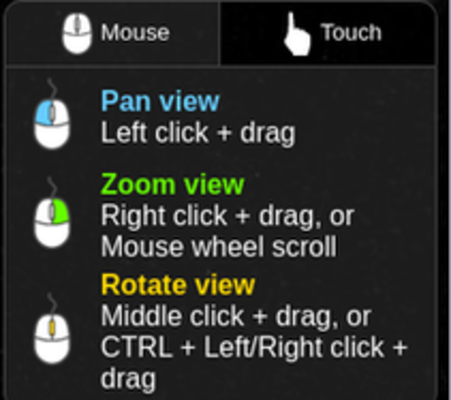
\includegraphics[width=4cm]{images/menus/souris.png}
}
\begin{figure}[ht]
\caption{\label{equiProj}\textit{Déplacements}}
\end{figure}
\end{center}
\newpage
\subsection{Visualisation des données}
Pour accéder à la plupart des options, le principe est le suivant. 
\begin{itemize}
\item {Affichage}
\begin{itemize}
\item Définir un rectangle de sélection	
	\begin{itemize}
	\item Touche {\tt Shift ($\big\Uparrow$)} du clavier + Touche gauche de la souris.
	\item Faire glisser la souris, pour définir une zone.
	\item Relâcher : la zone est sélectionnée, elle le sera tant qu'une autre zone ne sera pas définie.
	\item Optionnellement clic gauche en dehors de la zone pour faire disparaître l'affichage du rectangle de sélection.
	\end{itemize}
\item Choix dans le menu de gauche
    \begin{itemize}
	\item Sélectionner un item : {\tt S57 charts, Raster charts, Seabed charts,\ldots}
	\item Cocher un ou plusieurs sous-items : {\tt Depth area, Harbour area, \ldots}
	\item Cliquer sur le bouton : {\tt View/Refresh selection}
	\item Recommencer autant de fois que vous souhaitez avoir des informations nouvelles sur cette zone
	\end{itemize}
	\end{itemize}
	\item Suppression de l'affichage
    \begin{itemize}
	\item Désélectionner le/les item(s)  et/ou sous-item(s) à supprimer
	\item Cliquer sur le bouton : {\tt View/Refresh selection}
	\end{itemize}
\end{itemize}
%%%%%%%%%%%%%%%%%%%%%%%%%%%%%%%%%%%%%%%%%%%%%%%%%%%%%%%%%%%%%%%%%%%%%%%
\begin{center}
\framebox[1\width]{
	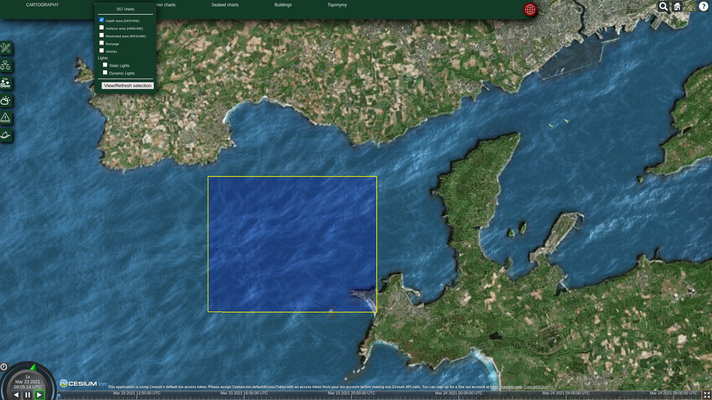
\includegraphics[width=16cm, height=9cm]{images/selection/selection_0.png}
}
\begin{figure}[ht]
\caption{\label{equiProj}\textit{Définition de la zone}}
\end{figure}
\end{center}
%%%%%%%%%%%%%%%%%%%%%%%%%%%%%%%%%%%%%%%%%%%%%%%%%%%%%%%%%%%%%%%%%%%%%%%
%%%%%%%%%%%%%%%%%%%%%%%%%%%%%%%%%%%%%%%%%%%%%%%%%%%%%%%%%%%%%%%%%%%%%%%
\begin{center}
\framebox[1\width]{
	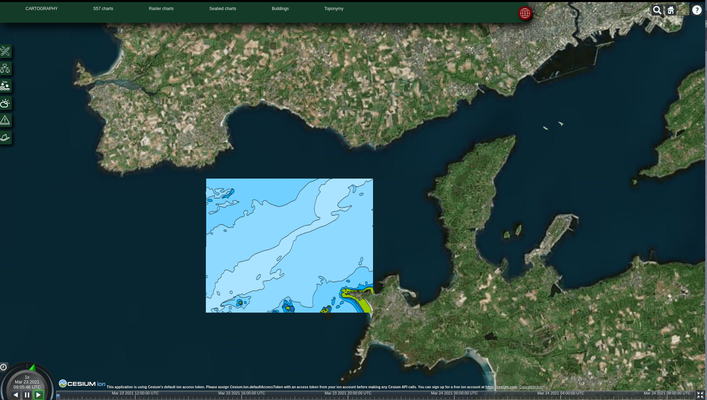
\includegraphics[width=16cm, height=8cm]{images/selection/selection_1.png}
}
\begin{figure}[ht]
\caption{\label{equiProj}\textit{Choix dans le menu, affichage}}
\end{figure}
\end{center}

%%%%%%%%%%%%%%%%%%%%%%%%%%%%%%%%%%%%%%%%%%%%%%%%%%%%%%%%%%%%%%%%%%%%%%%
\subsection{Les menus principaux}
%%%%%%%%%%%%%%%%%%%%%%%%%%%%%%%%%%%%%%%%%%%%%%%%%%%%%%%%%%%%%%%%%%%%%%%

\begin{center}
\framebox[1\width]{
	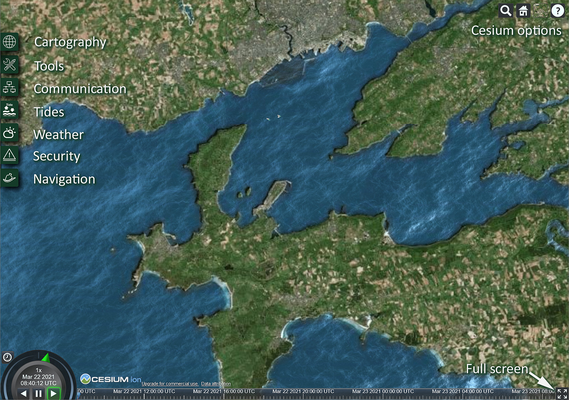
\includegraphics[width=16cm, height=8cm]{images/menus/menu_3.png}
}
\begin{figure}[ht]
\caption{\label{equiProj}\textit{Les deux menus principaux}}
\end{figure}
\end{center}
%%%%%%%%%%%%%%%%%%%%%%%%%%%%%%%%%%%%%%%%%%%%%%%%%%%%%%%%%%%%%%%%%%%%%%%
\newpage
\subsection{Les couches}
Toutes les données sont présentées dans des couches séparées et superposées. Il est ainsi possible de mixer les différentes informations.
%%%%%%%%%%%%%%%%%%%%%%%%%%%%%%%%%%%%%%%%%%%%%%%%%%%%%%%%%%%%%%%%%%%%%%%
\begin{center}
\framebox[1\width]{
	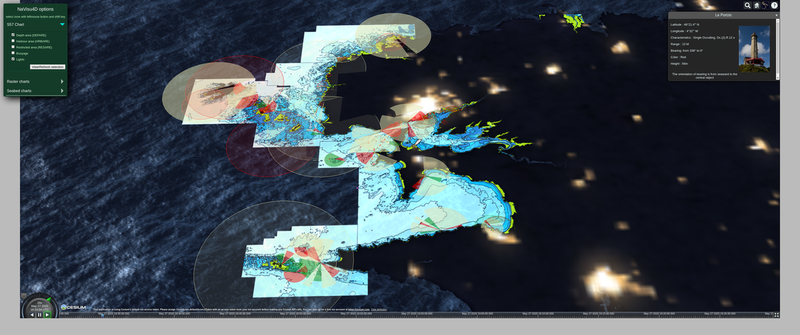
\includegraphics[width=15cm, height=8cm]{images/lights/lights_17.png}
}
\begin{figure}[ht]
\caption{\label{equiProj}\textit{Les feux,les amers et le balisage  S-57, imagerie satellite}}
\end{figure}
\end{center}
%%%%%%%%%%%%%%%%%%%%%%%%%%%%%%%%%%%%%%%%%%%%%%%%%%%%%%%%%%%%%%%%%%%%%%%
\chapter{Les outils}
\section{Coodonnées géographiques}
\subsection{Graticule}
%%%%%%%%%%%%%%%%%%%%%%%%%%%%%%%%%%%%%%%%%%%%%%%%%%%%%%%%%%%%%%%%%%%%%%%
\begin{center}
\framebox[1\width]{
	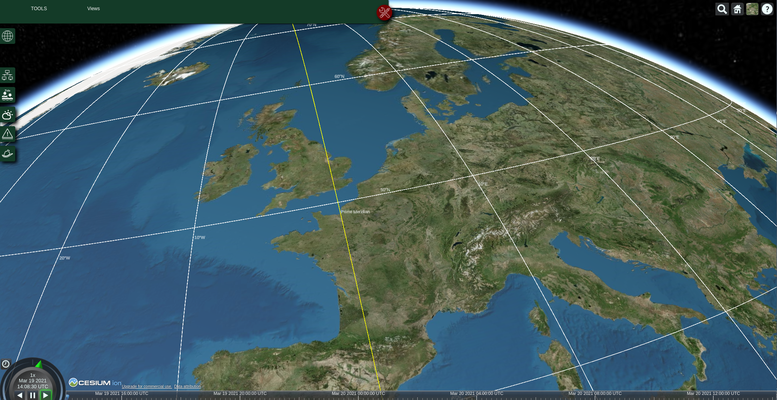
\includegraphics[width=15cm, height=8cm]{images/tools/graticule.png}
}
\begin{figure}[ht]
\caption{\label{graticule}\textit{Graticule}}
\end{figure}
\end{center}
\newpage
%%%%%%%%%%%%%%%%%%%%%%%%%%%%%%%%%%%%%%%%%%%%%%%%%%%%%%%%%%%%%%%%%%%%%%%
Ces données peuvent être affinées par l'item LatLon du menu  :
%%%%%%%%%%%%%%%%%%%%%%%%%%%%%%%%%%%%%%%%%%%%%%%%%%%%%%%%%%%%%%%%%%%%%%%
\begin{center}
\framebox[1\width]{
	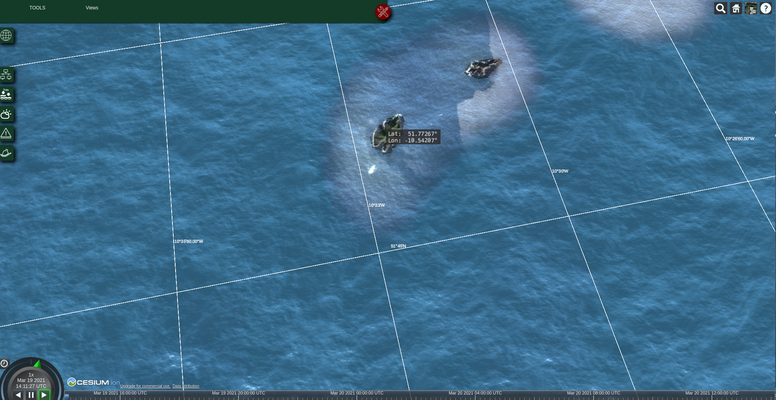
\includegraphics[width=15cm, height=8cm]{images/tools/latLon.png}
}
\begin{figure}[ht]
\caption{\label{graticule}\textit{Position en latitude longitude}}
\end{figure}
\end{center}
%%%%%%%%%%%%%%%%%%%%%%%%%%%%%%%%%%%%%%%%%%%%%%%%%%%%%%%%%%%%%%%%%%%%%%%
\section{Ecran multivues}
Il est possible d'avoir deux vues synchronisées d'un même endroit en cliquant sur l'item {\sc Views/View 2D/3D}.
La partie à gauche représente le modèle 3D tandis que la partie à droite montre la représentation cartographique 2D, plus classique.
%%%%%%%%%%%%%%%%%%%%%%%%%%%%%%%%%%%%%%%%%%%%%%%%%%%%%%%%%%%%%%%%%%%%%%%
\begin{center}
\framebox[1\width]{
	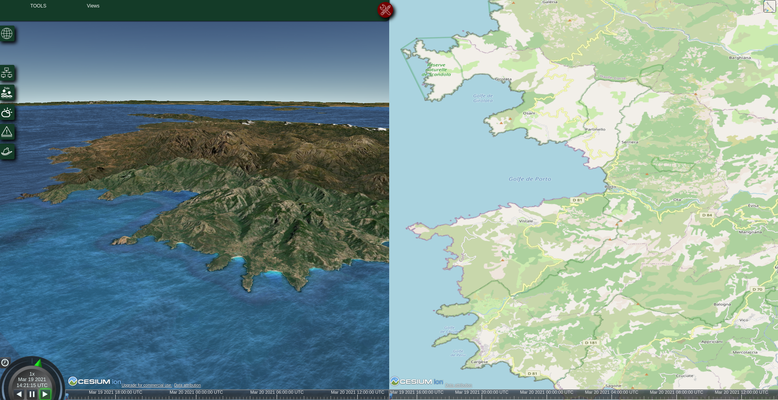
\includegraphics[width=15cm, height=8cm]{images/tools/2D3D.png}
}
\begin{figure}[ht]
\caption{\label{graticule}\textit{Deux représentations possibles}}
\end{figure}
\end{center}
%%%%%%%%%%%%%%%%%%%%%%%%%%%%%%%%%%%%%%%%%%%%%%%%%%%%%%%%%%%%%%%%%%%%%%%

%%%%%%%%%%%%%%%%%%%%%%%%%%%%%%%%%%%%%%%%%%%%%%%%%%%%%%%%%%%%%%%%%%%%%%%
\chapter{Imagerie et modèles numériques de terrain}
Le menu de droite permet de sélectionner différents types d'imageries projetées sur les modèles numériques de terrain : symboliques, orthophotos satellitaires ou aériennes.
%%%%%%%%%%%%%%%%%%%%%%%%%%%%%%%%%%%%%%%%%%%%%%%%%%%%%%%%%%%%%%%%%%%%%%%
\begin{center}
\framebox[1\width]{
	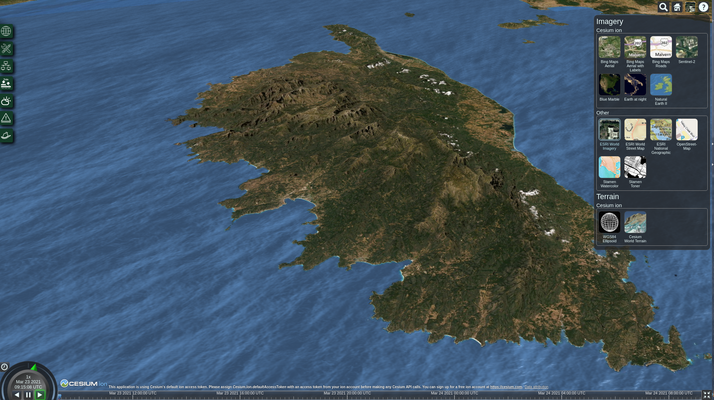
\includegraphics[width=16cm, height=8cm]{images/imagerie/esri.png}
}
\begin{figure}[ht]
\caption{\label{equiProj}\textit{Orthophotographie ESRI}}
\end{figure}
\end{center}
%%%%%%%%%%%%%%%%%%%%%%%%%%%%%%%%%%%%%%%%%%%%%%%%%%%%%%%%%%%%%%%%%%%%%%%
%%%%%%%%%%%%%%%%%%%%%%%%%%%%%%%%%%%%%%%%%%%%%%%%%%%%%%%%%%%%%%%%%%%%%%%
\begin{center}
\framebox[1\width]{
	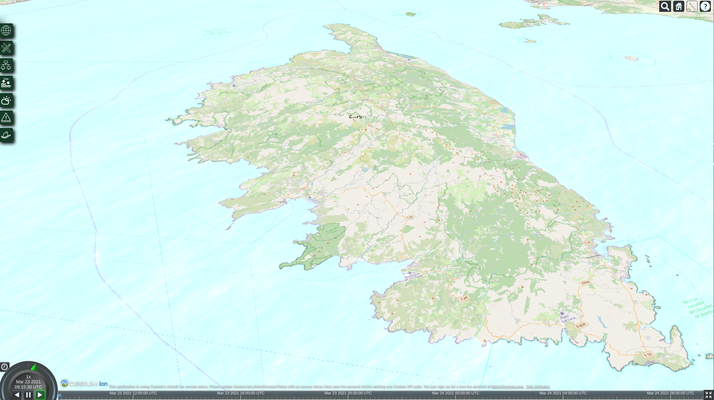
\includegraphics[width=16cm, height=9.5cm]{images/imagerie/osm.png}
}
\begin{figure}[ht]
\caption{\label{equiProj}\textit{Open Street Map}}
\end{figure}
\end{center}
%%%%%%%%%%%%%%%%%%%%%%%%%%%%%%%%%%%%%%%%%%%%%%%%%%%%%%%%%%%%%%%%%%%%%%%
%%%%%%%%%%%%%%%%%%%%%%%%%%%%%%%%%%%%%%%%%%%%%%%%%%%%%%%%%%%%%%%%%%%%%%%
\begin{center}
\framebox[1\width]{
	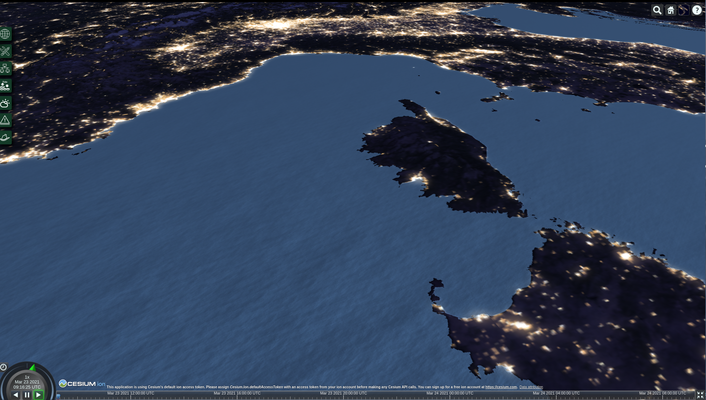
\includegraphics[width=16cm, height=9.5cm]{images/imagerie/night.png}
}
\begin{figure}[ht]
\caption{\label{equiProj}\textit{Image satellite }}
\end{figure}
\end{center}
%%%%%%%%%%%%%%%%%%%%%%%%%%%%%%%%%%%%%%%%%%%%%%%%%%%%%%%%%%%%%%%%%%%%%%%

\chapter{Cartographie}
Deux types de cartes sont présentes, les cartes raster et les cartes vectorielles, l'origine de ces cartes est le SHOM pour la France et la NOAA pour les Etats Unis. Concernant la France notre catalogue est pour le moment surtout centré sur la Mer d'Iroise en Bretagne (France).
\subsection{Cartes raster : GeoTIFF}
%%%%%%%%%%%%%%%%%%%%%%%%%%%%%%%%%%%%%%%%%%%%%%%%%%%%%%%%%%%%%%%%%%%%%%%
\begin{center}
\framebox[1\width]{
	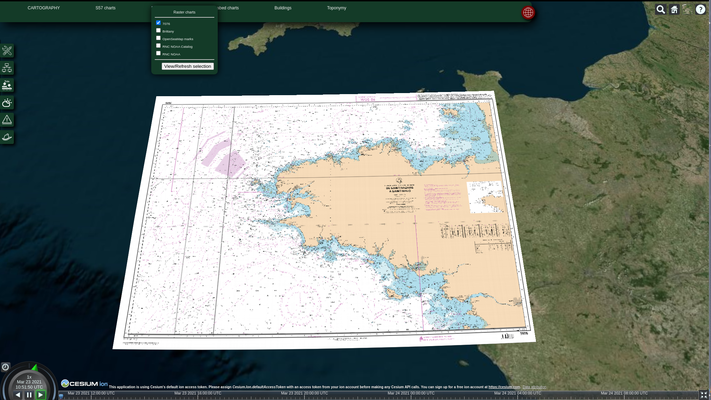
\includegraphics[width=14cm]{images/charts/raster_0.png}
}
\begin{figure}[ht]
\caption{\label{equiProj}\textit{Carte SHOM Numéro 7076}}
\end{figure}
\end{center}
%%%%%%%%%%%%%%%%%%%%%%%%%%%%%%%%%%%%%%%%%%%%%%%%%%%%%%%%%%%%%%%%%%%%%%%
%%%%%%%%%%%%%%%%%%%%%%%%%%%%%%%%%%%%%%%%%%%%%%%%%%%%%%%%%%%%%%%%%%%%%%%
\begin{center}
\framebox[1\width]{
	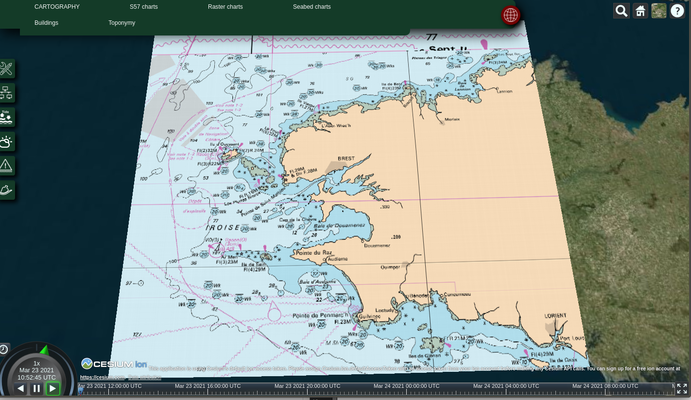
\includegraphics[width=14cm]{images/charts/raster_1.png}
}
\begin{figure}[ht]
\caption{\label{equiProj}\textit{Sélection d'une zone plus petite}}
\end{figure}
\end{center}
%%%%%%%%%%%%%%%%%%%%%%%%%%%%%%%%%%%%%%%%%%%%%%%%%%%%%%%%%%%%%%%%%%%%%%%
\subsection{Le balisage d'OpenSeaMap}
%%%%%%%%%%%%%%%%%%%%%%%%%%%%%%%%%%%%%%%%%%%%%%%%%%%%%%%%%%%%%%%%%%%%%%%
\begin{center}
\framebox[1\width]{
	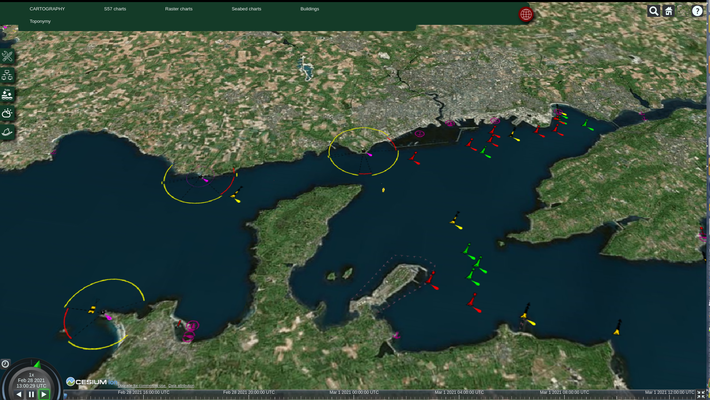
\includegraphics[width=14cm]{images/charts/openSeaMapMarks_ESRI.png}
}
\begin{figure}[ht]
\caption{\label{equiProj}\textit{OpenSeaMap marks avec la couche d'imagerie ESRI}}
\end{figure}
\end{center}
%%%%%%%%%%%%%%%%%%%%%%%%%%%%%%%%%%%%%%%%%%%%%%%%%%%%%%%%%%%%%%%%%%%%%%%
%%%%%%%%%%%%%%%%%%%%%%%%%%%%%%%%%%%%%%%%%%%%%%%%%%%%%%%%%%%%%%%%%%%%%%%
\begin{center}
\framebox[1\width]{
	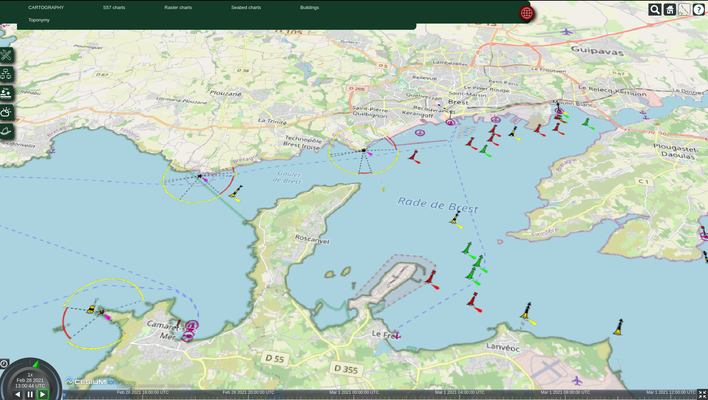
\includegraphics[width=14cm]{images/charts/openSeaMapMarks_OpenStreetMap.png}
}
\begin{figure}[ht]
\caption{\label{equiProj}\textit{OpenSeaMap marks avec la couche d'OpenStreetMap}}
\end{figure}
\end{center}
%%%%%%%%%%%%%%%%%%%%%%%%%%%%%%%%%%%%%%%%%%%%%%%%%%%%%%%%%%%%%%%%%%%%%%%
%%%%%%%%%%%%%%%%%%%%%%%%%%%%%%%%%%%%%%%%%%%%%%%%%%%%%%%%%%%%%%%%%%%%%%%
\begin{center}
\framebox[1\width]{
	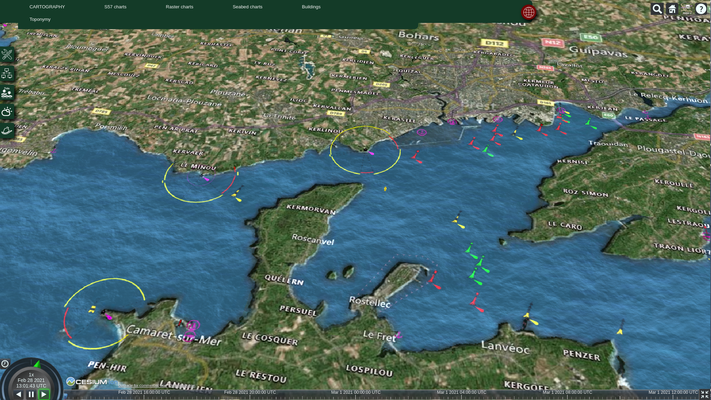
\includegraphics[width=14cm]{images/charts/openSeaMapMarks_BingMapLabels.png}
}
\begin{figure}[ht]
\caption{\label{equiProj}\textit{OpenSeaMap marks avec la couche d'imagerie Bing avec labels}}
\end{figure}
\end{center}
\newpage
%%%%%%%%%%%%%%%%%%%%%%%%%%%%%%%%%%%%%%%%%%%%%%%%%%%%%%%%%%%%%%%%%%%%%%%
\section{RNC Américaines}
%%%%%%%%%%%%%%%%%%%%%%%%%%%%%%%%%%%%%%%%%%%%%%%%%%%%%%%%%%%%%%%%%%%%%%%
Pour les Etats Unis, la NOAA met à la disposition du public différents services à la navigation, en particulier 
un serveur de cartographie tuilée : \\
\href{https://tileservice.charts.noaa.gov/tileset.html#50000\_1-locator}{https://tileservice.charts.noaa.gov/tileset.html\#50000\_1-locator}
%%%%%%%%%%%%%%%%%%%%%%%%%%%%%%%%%%%%%%%%%%%%%%%%%%%%%%%%%%%%%%%%%%%%%%%
\begin{center}
\framebox[1\width]{
	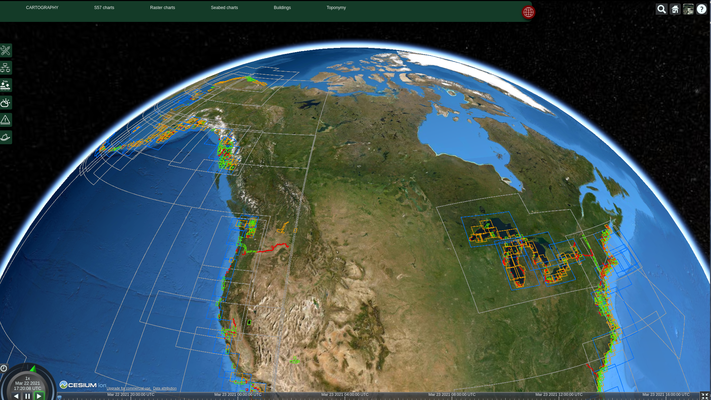
\includegraphics[width=14cm]{images/charts/noaa_4.png}
}
\begin{figure}[ht]
\caption{\label{equiProj}\textit{Le catalogue des cartes raster de la NOAA}}
\end{figure}
\end{center}
%%%%%%%%%%%%%%%%%%%%%%%%%%%%%%%%%%%%%%%%%%%%%%%%%%%%%%%%%%%%%%%%%%%%%%%
%%%%%%%%%%%%%%%%%%%%%%%%%%%%%%%%%%%%%%%%%%%%%%%%%%%%%%%%%%%%%%%%%%%%%%%
\begin{center}
\framebox[1\width]{
	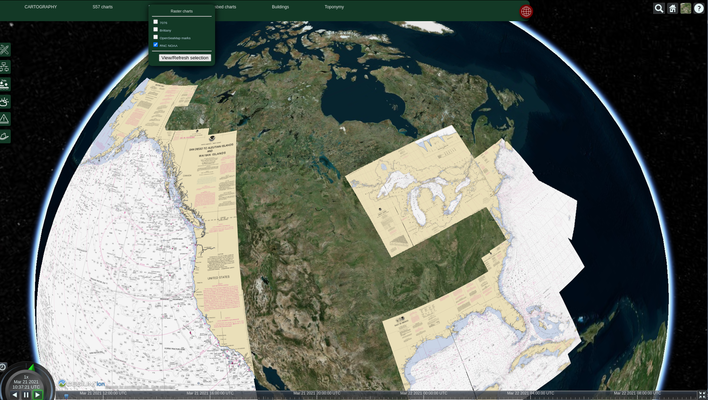
\includegraphics[width=14cm]{images/charts/noaa_0.png}
}
\begin{figure}[ht]
\caption{\label{equiProj}\textit{Couverture des cartes raster de la NOAA}}
\end{figure}
\end{center}
%%%%%%%%%%%%%%%%%%%%%%%%%%%%%%%%%%%%%%%%%%%%%%%%%%%%%%%%%%%%%%%%%%%%%%%
%%%%%%%%%%%%%%%%%%%%%%%%%%%%%%%%%%%%%%%%%%%%%%%%%%%%%%%%%%%%%%%%%%%%%%%
\begin{center}
\framebox[1\width]{
	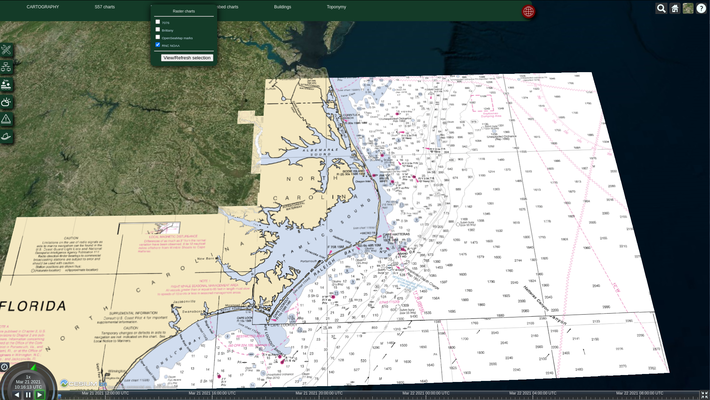
\includegraphics[width=14cm]{images/charts/noaa_1.png}
}
\begin{figure}[ht]
\caption{\label{equiProj}\textit{Détail d'une des cartes}}
\end{figure}
\end{center}
%%%%%%%%%%%%%%%%%%%%%%%%%%%%%%%%%%%%%%%%%%%%%%%%%%%%%%%%%%%%%%%%%%%%%%%
%%%%%%%%%%%%%%%%%%%%%%%%%%%%%%%%%%%%%%%%%%%%%%%%%%%%%%%%%%%%%%%%%%%%%%%
\begin{center}
\framebox[1\width]{
	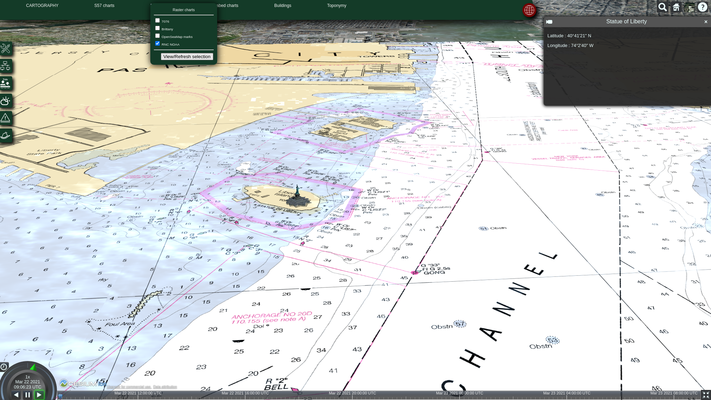
\includegraphics[width=14cm]{images/charts/noaa_2.png}
}
\begin{figure}[ht]
\caption{\label{equiProj}\textit{Détail d'une des cartes}}
\end{figure}
\end{center}
%%%%%%%%%%%%%%%%%%%%%%%%%%%%%%%%%%%%%%%%%%%%%%%%%%%%%%%%%%%%%%%%%%%%%%%
\newpage
%%%%%%%%%%%%%%%%%%%%%%%%%%%%%%%%%%%%%%%%%%%%%%%%%%%%%%%%%%%%%%%%%%%%%%%
\section{Cartographie personnalisée}
%%%%%%%%%%%%%%%%%%%%%%%%%%%%%%%%%%%%%%%%%%%%%%%%%%%%%%%%%%%%%%%%%%%%%%%
Il est possible de posséder des cartes personnelles qui ne seront pas partagées.
%%%%%%%%%%%%%%%%%%%%%%%%%%%%%%%%%%%%%%%%%%%%%%%%%%%%%%%%%%%%%%%%%%%%%%%
\begin{center}
\framebox[1\width]{
	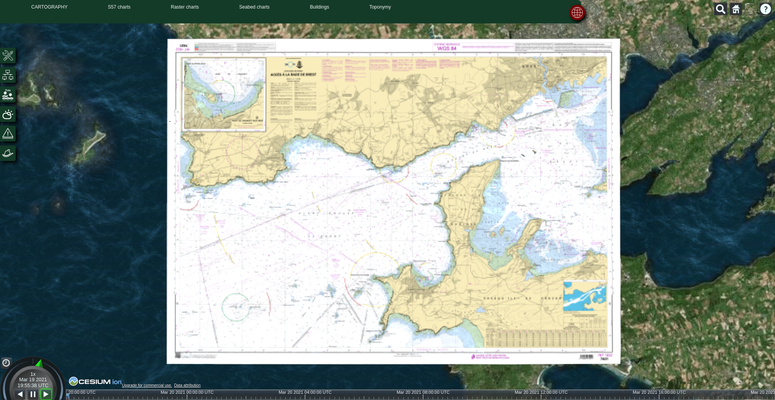
\includegraphics[width=14cm]{images/charts/raster_4.png}
}
\begin{figure}[ht]
\caption{\label{equiProj}\textit{La carte raster 7401 du Shom}}
\end{figure}
\end{center}
%%%%%%%%%%%%%%%%%%%%%%%%%%%%%%%%%%%%%%%%%%%%%%%%%%%%%%%%%%%%%%%%%%%%%%%
%%%%%%%%%%%%%%%%%%%%%%%%%%%%%%%%%%%%%%%%%%%%%%%%%%%%%%%%%%%%%%%%%%%%%%%
\begin{center}
\framebox[1\width]{
	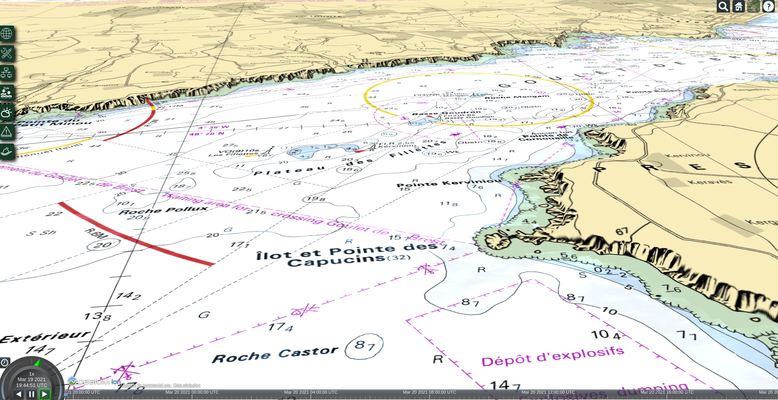
\includegraphics[width=14cm]{images/charts/raster_2.png}
}
\begin{figure}[ht]
\caption{\label{equiProj}\textit{La carte 7401 en 3D}}
\end{figure}
\end{center}
%%%%%%%%%%%%%%%%%%%%%%%%%%%%%%%%%%%%%%%%%%%%%%%%%%%%%%%%%%%%%%%%%%%%%%%
%%%%%%%%%%%%%%%%%%%%%%%%%%%%%%%%%%%%%%%%%%%%%%%%%%%%%%%%%%%%%%%%%%%%%%%
\begin{center}
\framebox[1\width]{
	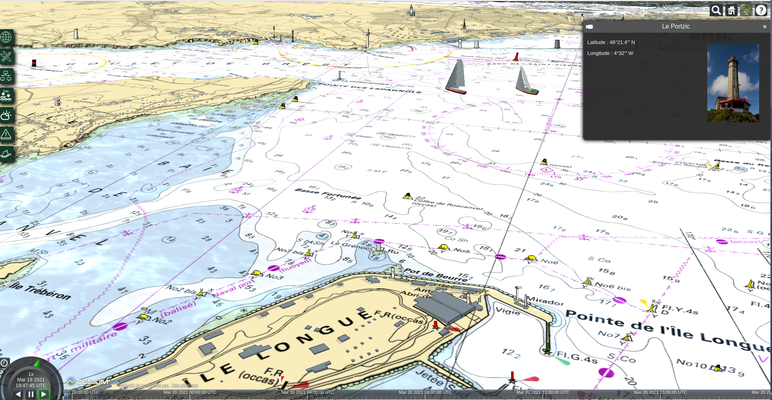
\includegraphics[width=14cm]{images/charts/raster_3.png}
}
\begin{figure}[ht]
\caption{\label{equiProj}\textit{Fusion avec les éléments de balisage de S57}}
\end{figure}
\end{center}
%%%%%%%%%%%%%%%%%%%%%%%%%%%%%%%%%%%%%%%%%%%%%%%%%%%%%%%%%%%%%%%%%%%%%%%

\subsection{Cartes vectorielles : S-57}
L'intérêt de ces cartes, réside dans le fait que chaque information : balisage, sondes, zones particulières, \ldots\hspace{.1cm} peut être extraite de la base de données et présentée de façon individuelle, pouvant ainsi répondre aux interrogations de l'utilisateur. Pour ce démonstrateur seules les Depth Area (DEPARE), les Harbour Area (HRBARE), les Restricted Area (RESARE), le balisage et les amers sont visualisés, mais l'ensemble des objets S-57 et de leurs attributs sont en bases de données et accessibles.
%%%%%%%%%%%%%%%%%%%%%%%%%%%%%%%%%%%%%%%%%%%%%%%%%%%%%%%%%%%%%%%%%%%%%%%
\begin{center}
\framebox[1\width]{
	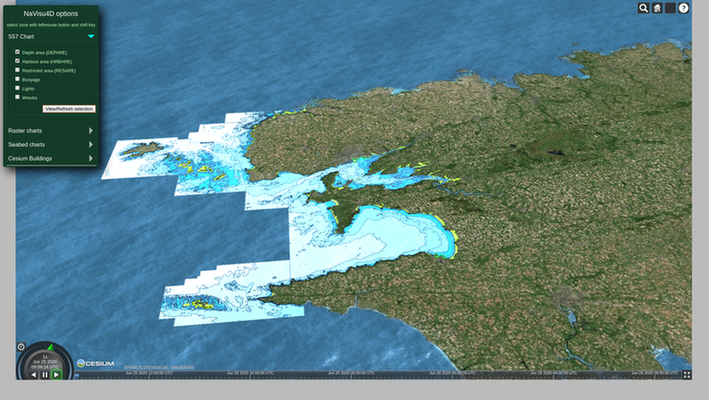
\includegraphics[width=14cm]{images/charts/s57_0.png}
}
\begin{figure}[ht]
\caption{\label{equiProj}\textit{Assemblage de différentes cartes S-57}}
\end{figure}
\end{center}
%%%%%%%%%%%%%%%%%%%%%%%%%%%%%%%%%%%%%%%%%%%%%%%%%%%%%%%%%%%%%%%%%%%%%%%
%%%%%%%%%%%%%%%%%%%%%%%%%%%%%%%%%%%%%%%%%%%%%%%%%%%%%%%%%%%%%%%%%%%%%%%
\begin{center}
\framebox[1\width]{
	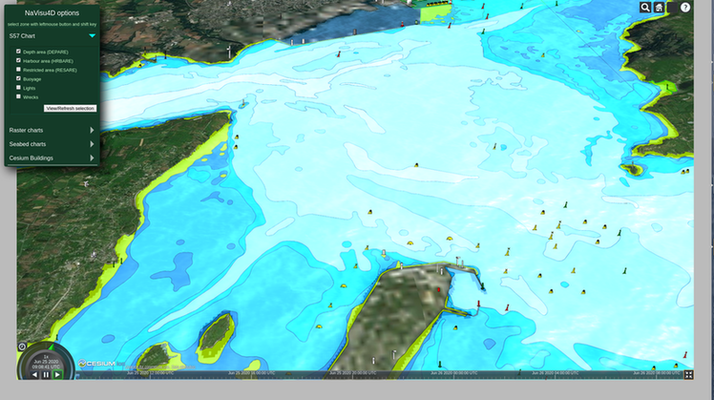
\includegraphics[width=14cm]{images/charts/s57_1.png}
}
\begin{figure}[ht]
\caption{\label{equiProj}\textit{Détails d'une zone plus petite, isobathes + balisage en rade de Brest}}
\end{figure}
\end{center}
%%%%%%%%%%%%%%%%%%%%%%%%%%%%%%%%%%%%%%%%%%%%%%%%%%%%%%%%%%%%%%%%%%%%%%%
%%%%%%%%%%%%%%%%%%%%%%%%%%%%%%%%%%%%%%%%%%%%%%%%%%%%%%%%%%%%%%%%%%%%%%%
\begin{center}
\framebox[1\width]{
	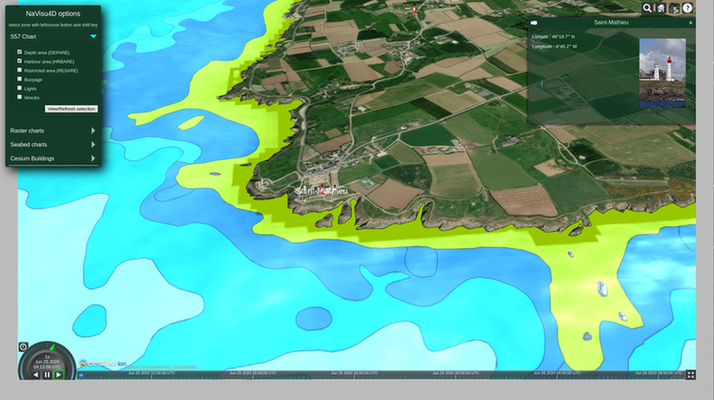
\includegraphics[width=16cm]{images/charts/s57_2.png}
}
\begin{figure}[ht]
\caption{\label{equiProj}\textit{L'utilisateur peut interroger chaque objet}}
\end{figure}
\end{center}

%%%%%%%%%%%%%%%%%%%%%%%%%%%%%%%%%%%%%%%%%%%%%%%%%%%%%%%%%%%%%%%%%%%%%%%

\section{Les feux}
\subsection{Option statique des feux}
%%%%%%%%%%%%%%%%%%%%%%%%%%%%%%%%%%%%%%%%%%%%%%%%%%%%%%%%%%%%%%%%%%%%%%%
Comme sur les cartes classiques 2D, les feux sont affichés en fonction de leur portée, un clic sur ces feux 
affiche leurs attributs.
\begin{center}
\framebox[1\width]{
	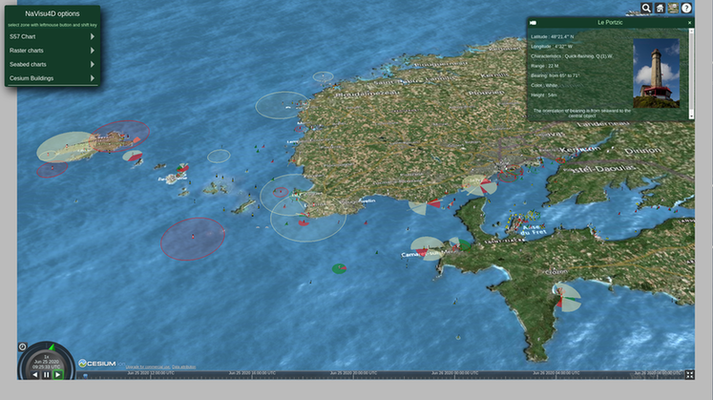
\includegraphics[width=15cm]{images/charts/s57_3.png}
}
\begin{figure}[ht]
\caption{\label{equiProj}\textit{Les feux}}
\end{figure}
\end{center}
%%%%%%%%%%%%%%%%%%%%%%%%%%%%%%%%%%%%%%%%%%%%%%%%%%%%%%%%%%%%%%%%%%%%%%%
\subsection{Option dynamique des feux}
%%%%%%%%%%%%%%%%%%%%%%%%%%%%%%%%%%%%%%%%%%%%%%%%%%%%%%%%%%%%%%%%%%%%%%%
Les caractéristiques statiques et dynamiques sont ici prises en compte pour la simulation\\
 (type, période, groupe, \ldots)
\begin{center}
\framebox[1\width]{
	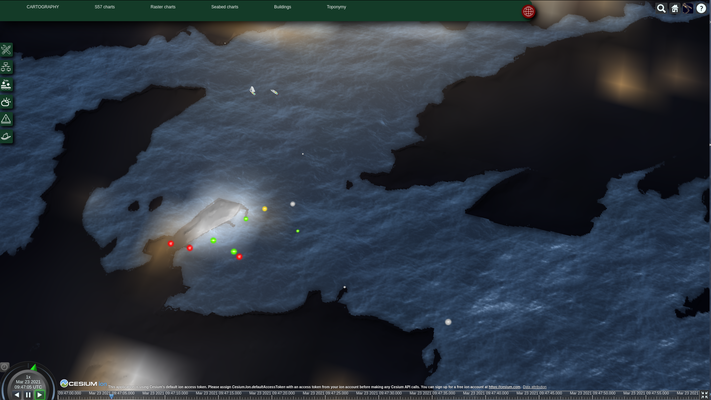
\includegraphics[width=15cm]{images/lights/feux_dyna.png}
}
\begin{figure}[ht]
\caption{\label{equiProj}\textit{Les feux, option dynamique (une partie de la Rade de Brest)}}
\end{figure}
\end{center}
%%%%%%%%%%%%%%%%%%%%%%%%%%%%%%%%%%%%%%%%%%%%%%%%%%%%%%%%%%%%%%%%%%%%%%%

%%%%%%%%%%%%%%%%%%%%%%%%%%%%%%%%%%%%%%%%%%%%%%%%%%%%%%%%%%%%%%%%%%%%%%%
\begin{center}
\framebox[1\width]{
	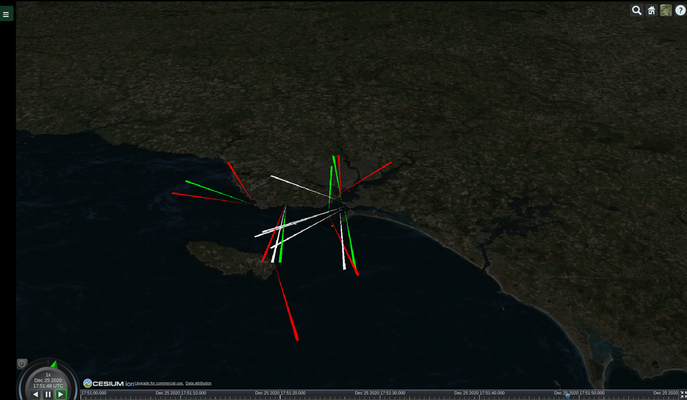
\includegraphics[width=16cm]{images/lights/feux_dyna_secteurs.png}
}
\begin{figure}[ht]
\caption{\label{equiProj}\textit{Les feux à secteurs (entrée de Lorient)}}
\end{figure}
\end{center}
%%%%%%%%%%%%%%%%%%%%%%%%%%%%%%%%%%%%%%%%%%%%%%%%%%%%%%%%%%%%%%%%%%%%%%%
Il est évidemment possible de superposer les deux modes.
%%%%%%%%%%%%%%%%%%%%%%%%%%%%%%%%%%%%%%%%%%%%%%%%%%%%%%%%%%%%%%%%%%%%%%%
\begin{center}
\framebox[1\width]{
	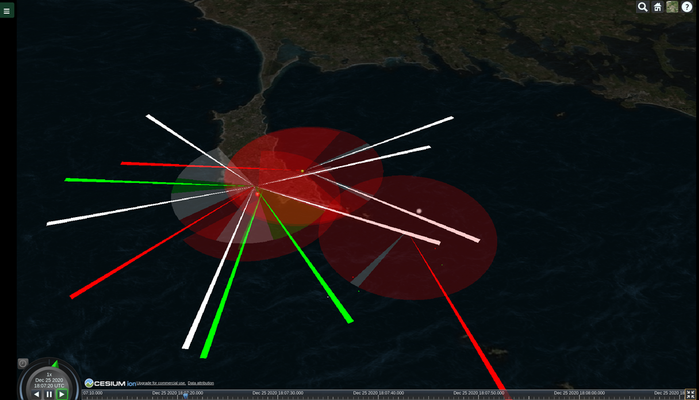
\includegraphics[width=16cm]{images/lights/feux_dyna_stat.png}
}
\begin{figure}[ht]
\caption{\label{equiProj}\textit{Les feux à secteurs, options statique et dynamique  (La Teignouse)}}
\end{figure}
\end{center}
%%%%%%%%%%%%%%%%%%%%%%%%%%%%%%%%%%%%%%%%%%%%%%%%%%%%%%%%%%%%%%%%%%%%%%%
\section{Toponymie}
Le SHOM met à disposition les toponymes marins et côtiers à l'échelle mondiale. Ces toponymes sont issus des cartes ENC.
{\small
\begin{verbatim}
FR301020,FR303150,FR303160,FR303180,FR303190,FR166230,FR200010,FR474170,FR270140,
FR571230-FR402050, FR301010, FR301030, FR301040, FR302030, FR302040, FR302050, 
FR302080, FR302090, FR303010, FR303030, FR303040, FR366800, FR368240, FR368570, 
FR369300, FR369400, FR369410, FR369510, FR369660, FR370080, FR370250, FR370660,
FR370670, FR370680, FR370690, FR402040, FR475940,FR277510,FR276250,FR353010,FR274750,
FR332010,FR374850,FR374840,FR366860,FR367680,FR370520,FR469850,FR470510,
FR473130,FR473200,FR473750,FR371710-FR360330,FR369550,FR473730,FR473720,
FR473550,FR473540,FR473520,FR47353H,FR266880,FR266890,FR266900,FR266910,
FR266920-FR274860,FR476790,FR476780,FR335010
\end{verbatim}
}
%%%%%%%%%%%%%%%%%%%%%%%%%%%%%%%%%%%%%%%%%%%%%%%%%%%%%%%%%%%%%%%%%%%%%%%
\begin{center}
\framebox[1\width]{
	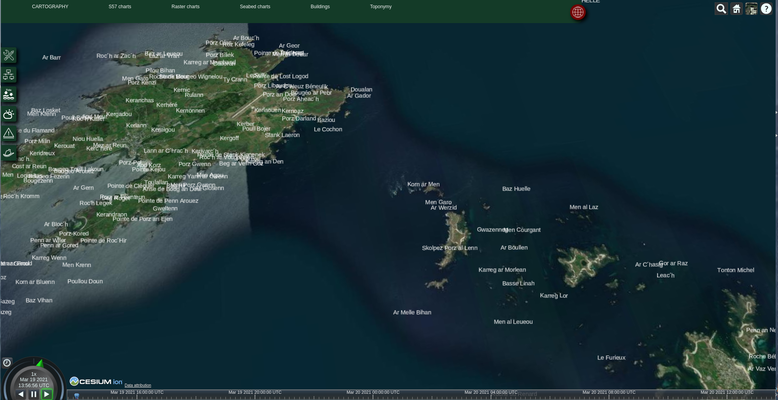
\includegraphics[width=16cm]{images/charts/toponymes.png}
}
\begin{figure}[ht]
\caption{\label{toponymes}\textit{Toponymes}}
\end{figure}
\end{center}
%%%%%%%%%%%%%%%%%%%%%%%%%%%%%%%%%%%%%%%%%%%%%%%%%%%%%%%%%%%%%%%%%%%%%%%
Cette option, peut aussi être compléter par la couche "Bing Maps, Aerial with labels". Ou la couche OpenStreetMap.
%%%%%%%%%%%%%%%%%%%%%%%%%%%%%%%%%%%%%%%%%%%%%%%%%%%%%%%%%%%%%%%%%%%%%%%
\begin{center}
\framebox[1\width]{
	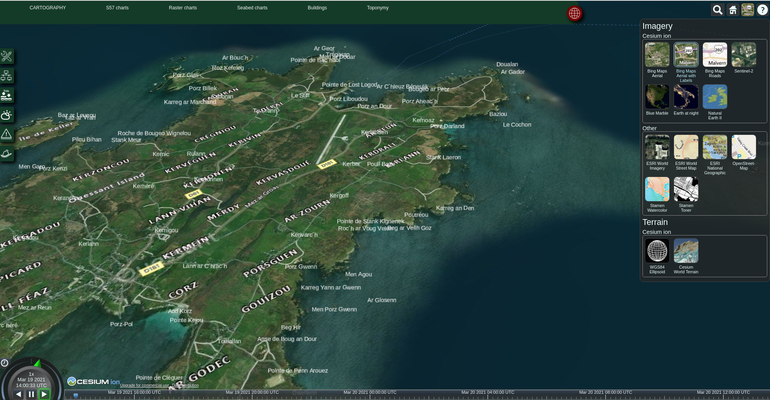
\includegraphics[width=16cm]{images/charts/toponymes_1.png}
}
\begin{figure}[ht]
\caption{\label{toponymes}\textit{Toponymes}}
\end{figure}
\end{center}
%%%%%%%%%%%%%%%%%%%%%%%%%%%%%%%%%%%%%%%%%%%%%%%%%%%%%%%%%%%%%%%%%%%%%%%
\chapter{La sécurité}
\section{Les Avis Urgents aux navigateurs  ({\sc Avurnav})}
En France métropolitaine,la Préfecture maritime  publie des avis urgents aux navigateurs : 
\begin{center}
\begin{minipage}{14cm}
\href{https://www.premar-manche.gouv.fr/avis-urgents-aux-navigateurs}{https://www.premar-manche.gouv.fr/avis-urgents-aux-navigateurs}\\
\href{https://www.premar-atlantique.gouv.fr/avis-urgents-aux-navigateurs}{https://www.premar-atlantique.gouv.fr/avis-urgents-aux-navigateurs}\\
\href{https://www.premar-mediterranee.gouv.fr/avis-urgents-aux-navigateurs}{https://www.premar-mediterranee.gouv.fr/avis-urgents-aux-navigateurs}
\end{minipage}
\end{center}
Depuis le menu {\tt Security} il est possible d'afficher les icones corespondantes aux avurnav actifs. Un clic sur une icone permet l'affichage du détail des informations.
%%%%%%%%%%%%%%%%%%%%%%%%%%%%%%%%%%%%%%%%%%%%%%%%%%%%%%%%%%%%%%%%%%%%%%%
\begin{center}
\framebox[1\width]{
	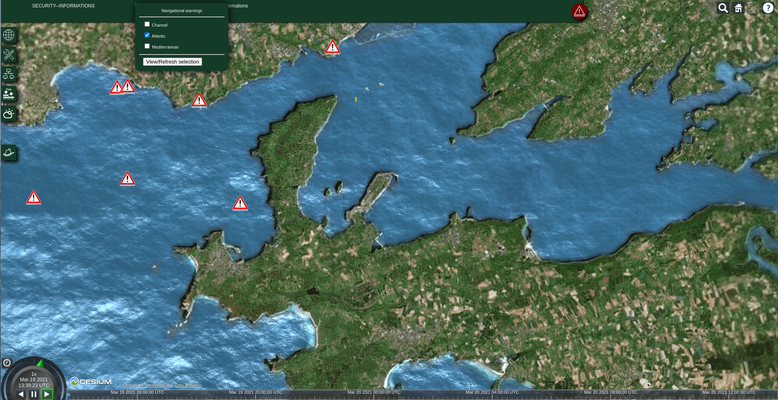
\includegraphics[width=15cm, height=8cm]{images/security/avurnav_0.png}
}
\begin{figure}[ht]
\caption{\label{equiProj}\textit{Affichage des Avurnav actifs}}
\end{figure}
\end{center}
%%%%%%%%%%%%%%%%%%%%%%%%%%%%%%%%%%%%%%%%%%%%%%%%%%%%%%%%%%%%%%%%%%%%%%%
\begin{center}
\framebox[1\width]{
	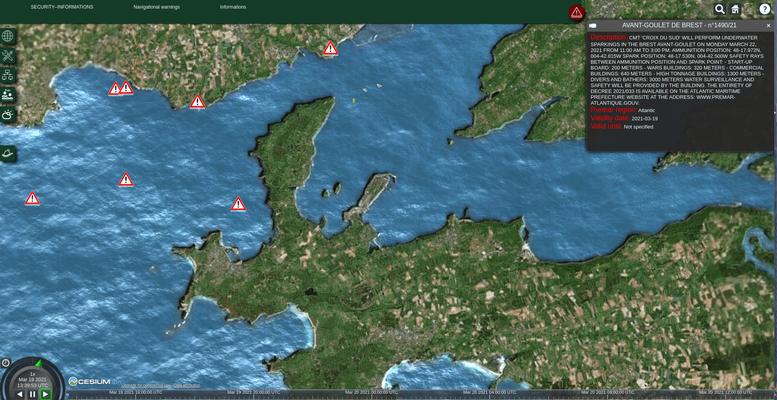
\includegraphics[width=15cm, height=8cm]{images/security/avurnav_1.png}
}
\begin{figure}[ht]
\caption{\label{equiProj}\textit{Affichage du texte d'un avis particulier}}
\end{figure}
\end{center}
%%%%%%%%%%%%%%%%%%%%%%%%%%%%%%%%%%%%%%%%%%%%%%%%%%%%%%%%%%%%%%%%%%%%%%%
\chapter{Les marées}
\section{Marégrammes du Shom}
Pour un certain nombre de ports Français, le Shom met à disposition les prédictions de marée pour quatre jours.
Ainsi que des informations météorologiques et de mer.
%%%%%%%%%%%%%%%%%%%%%%%%%%%%%%%%%%%%%%%%%%%%%%%%%%%%%%%%%%%%%%%%%%%%%%%
\begin{center}
\framebox[1\width]{
	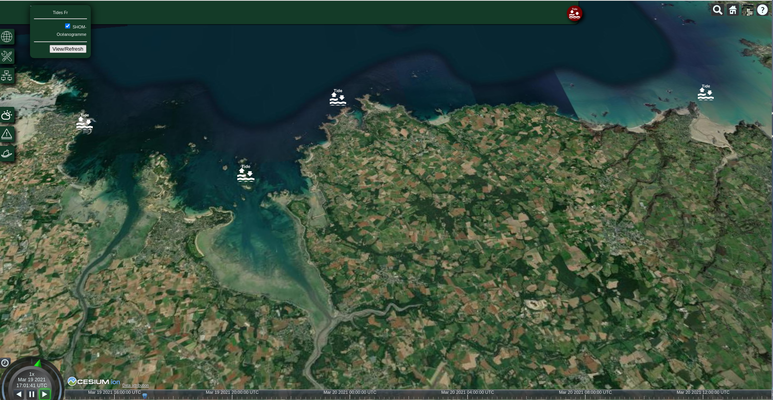
\includegraphics[width=15cm, height=8cm]{images/tides/maree_0.png}
}
\begin{figure}[ht]
\caption{\label{equiProj}\textit{Les icones de marée}}
\end{figure}
\end{center}
%%%%%%%%%%%%%%%%%%%%%%%%%%%%%%%%%%%%%%%%%%%%%%%%%%%%%%%%%%%%%%%%%%%%%%%
%%%%%%%%%%%%%%%%%%%%%%%%%%%%%%%%%%%%%%%%%%%%%%%%%%%%%%%%%%%%%%%%%%%%%%%
\begin{center}
\framebox[1\width]{
	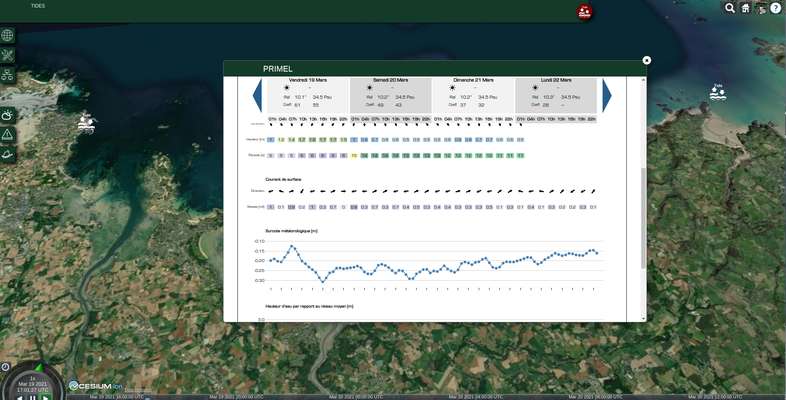
\includegraphics[width=15cm, height=8cm]{images/tides/maree_1.png}
}
\begin{figure}[ht]
\caption{\label{equiProj}\textit{Affichage d'un marégramme}}
\end{figure}
\end{center}
%%%%%%%%%%%%%%%%%%%%%%%%%%%%%%%%%%%%%%%%%%%%%%%%%%%%%%%%%%%%%%%%%%%%%%%
\chapter{La météo}
\section{Météo marine}
%%%%%%%%%%%%%%%%%%%%%%%%%%%%%%%%%%%%%%%%%%%%%%%%%%%%%%%%%%%%%%%%%%%%%%%
\begin{center}
\framebox[1\width]{
	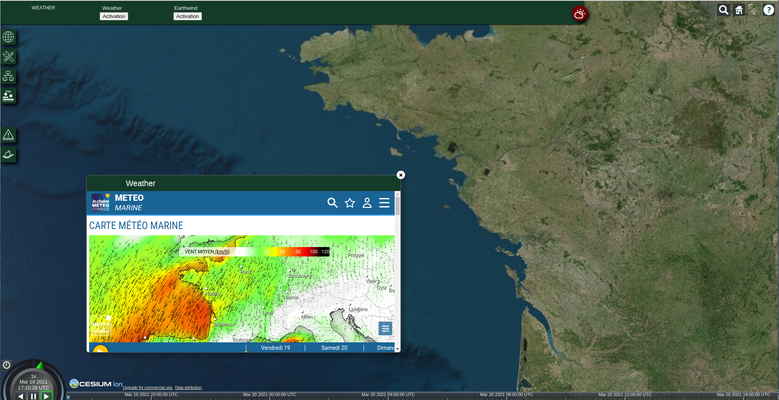
\includegraphics[width=15cm, height=8cm]{images/forecast/meteo_0.png}
}
\begin{figure}[ht]
\caption{\label{equiProj}\textit{METEO {\sc marine}}}
\end{figure}
\end{center}
%%%%%%%%%%%%%%%%%%%%%%%%%%%%%%%%%%%%%%%%%%%%%%%%%%%%%%%%%%%%%%%%%%%%%%%

%%%%%%%%%%%%%%%%%%%%%%%%%%%%%%%%%%%%%%%%%%%%%%%%%%%%%%%%%%%%%%%%%%%%%%%
\chapter{La bathymétrie}
%%%%%%%%%%%%%%%%%%%%%%%%%%%%%%%%%%%%%%%%%%%%%%%%%%%%%%%%%%%%%%%%%%%%%%%
\begin{center}
\framebox[1\width]{
	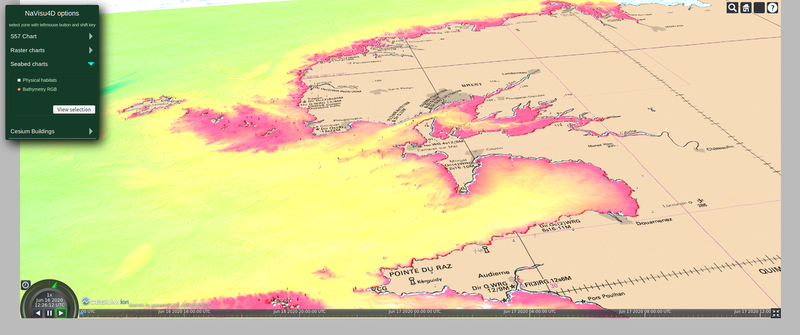
\includegraphics[width=15cm, height=8cm]{images/bathy/emodnet_1.png}
}
\begin{figure}[ht]
\caption{\label{equiProj}\textit{Image GeoTIFF du projet EMODnet}}
\end{figure}
\end{center}
%%%%%%%%%%%%%%%%%%%%%%%%%%%%%%%%%%%%%%%%%%%%%%%%%%%%%%%%%%%%%%%%%%%%%%%
\section{Bathymétrie locale}
Il est possible d'afficher des données de sondes personnalisées. Dans ce cas les données sont des valeurs de sondes mesurées par l'utilisateur. Ces sondes sont mises au format csv, par exemple. Elles sont ensuite transformées, puis intégrées à l'univers virtuel pour visualisation. Ici aussi l'utilisateur de l'application peut interroger ces données.
%%%%%%%%%%%%%%%%%%%%%%%%%%%%%%%%%%%%%%%%%%%%%%%%%%%%%%%%%%%%%%%%%%%%%%%
\begin{center}
\framebox[1\width]{
	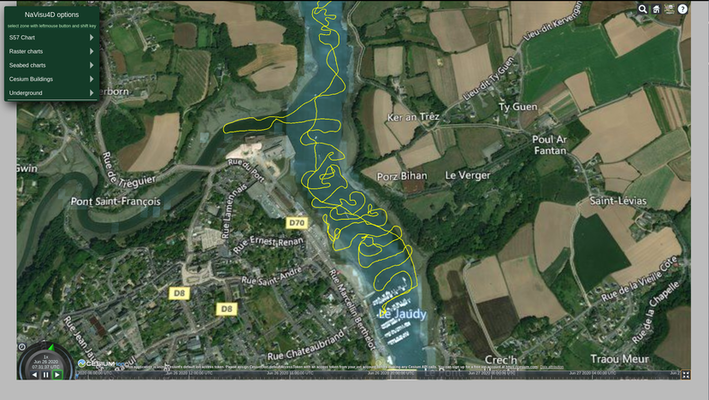
\includegraphics[width=14cm]{images/bathy/estran_0.png}
}
\begin{figure}[ht]
\caption{\label{equiProj}\textit{Sondes bathymétriques personnelles : affichage}}
\end{figure}
\end{center}
%%%%%%%%%%%%%%%%%%%%%%%%%%%%%%%%%%%%%%%%%%%%%%%%%%%%%%%%%%%%%%%%%%%%%%%
%%%%%%%%%%%%%%%%%%%%%%%%%%%%%%%%%%%%%%%%%%%%%%%%%%%%%%%%%%%%%%%%%%%%%%%
\begin{center}
\framebox[1\width]{
	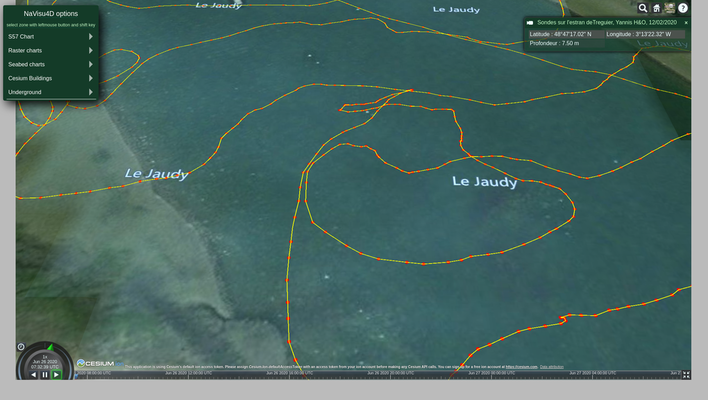
\includegraphics[width=14cm]{images/bathy/estran_1.png}
}
\begin{figure}[ht]
\caption{\label{equiProj}\textit{Sondes bathymétriques personnelles : interrogation}}
\end{figure}
\end{center}
%%%%%%%%%%%%%%%%%%%%%%%%%%%%%%%%%%%%%%%%%%%%%%%%%%%%%%%%%%%%%%%%%%%%%%%
\section{Bathymétrie WMS}
Plusieurs serveurs Web services permettent d'accéder aux images de la bathymétrie. Pour le moment \nav permet l'accès aux services raster : EMODnet, Homonim et Litto3D. En parallèle nous préparons l'accès simultané aux véritables valeurs de sonde.
\subsection{Bathymétrie EMODnet}
%%%%%%%%%%%%%%%%%%%%%%%%%%%%%%%%%%%%%%%%%%%%%%%%%%%%%%%%%%%%%%%%%%%%%%%
\begin{center}
\framebox[1\width]{
	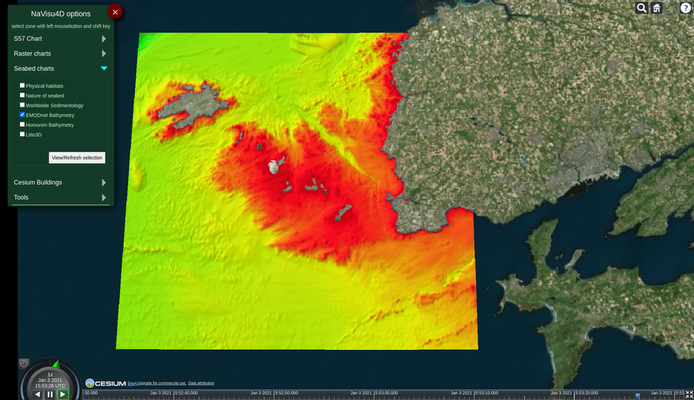
\includegraphics[width=14cm]{images/bathy/bathyEmodnet.png}
}
\begin{figure}[ht]
\caption{\label{bathyEmodnet}\textit{WMS Bathymétrie EMODnet}}
\end{figure}
\end{center}
%%%%%%%%%%%%%%%%%%%%%%%%%%%%%%%%%%%%%%%%%%%%%%%%%%%%%%%%%%%%%%%%%%%%%%%
\subsection{Bathymétrie Homonim}
%%%%%%%%%%%%%%%%%%%%%%%%%%%%%%%%%%%%%%%%%%%%%%%%%%%%%%%%%%%%%%%%%%%%%%%
\begin{center}
\framebox[1\width]{
	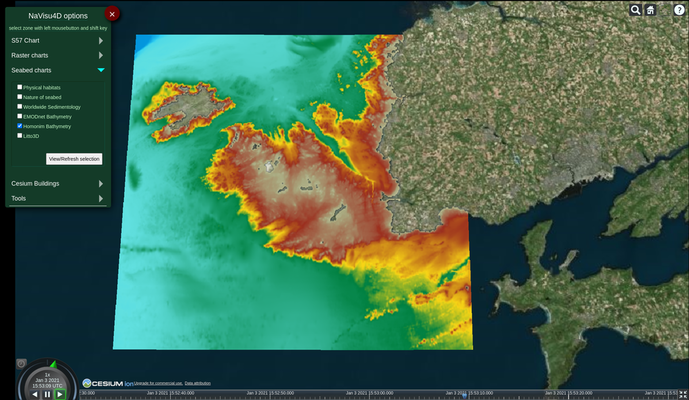
\includegraphics[width=14cm]{images/bathy/bathyHomonim.png}
}
\begin{figure}[ht]
\caption{\label{bathyHomonim}\textit{WMS Bathymétrie Homonim}}
\end{figure}
\end{center}
%%%%%%%%%%%%%%%%%%%%%%%%%%%%%%%%%%%%%%%%%%%%%%%%%%%%%%%%%%%%%%%%%%%%%%%
\subsection{Bathymétrie Litto3D}
%%%%%%%%%%%%%%%%%%%%%%%%%%%%%%%%%%%%%%%%%%%%%%%%%%%%%%%%%%%%%%%%%%%%%%%
\begin{center}
\framebox[1\width]{
	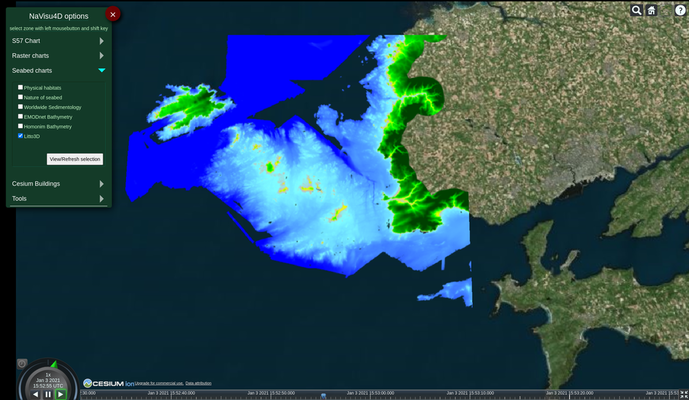
\includegraphics[width=14cm]{images/bathy/bathyLitto3D.png}
}
\begin{figure}[ht]
\caption{\label{bathyLitto3D}\textit{WMS Bathymétrie Litto3D}}
\end{figure}
\end{center}
%%%%%%%%%%%%%%%%%%%%%%%%%%%%%%%%%%%%%%%%%%%%%%%%%%%%%%%%%%%%%%%%%%%%%%%
\section{les points d'intérêt}
Il est possible de représenter des points particuliers, ici des épaves et de leur associer des informations : images, sons, vidéos
%%%%%%%%%%%%%%%%%%%%%%%%%%%%%%%%%%%%%%%%%%%%%%%%%%%%%%%%%%%%%%%%%%%%%%%
\begin{center}
\framebox[1\width]{
	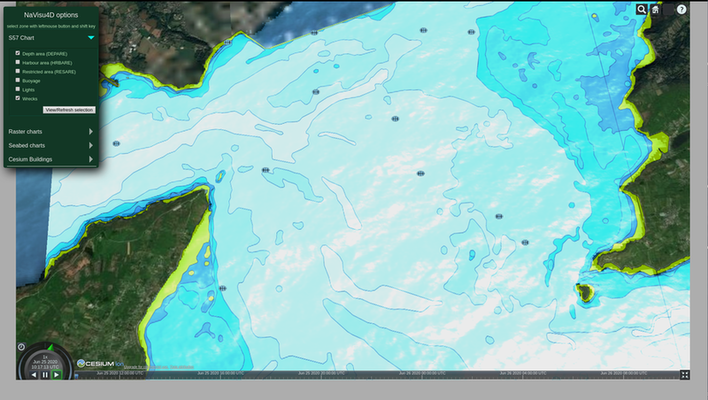
\includegraphics[width=15cm]{images/epaves/epave_0.png}
}
\begin{figure}[ht]
\caption{\label{equiProj}\textit{Extrait de la base de données du SHOM}}
\end{figure}
\end{center}
%%%%%%%%%%%%%%%%%%%%%%%%%%%%%%%%%%%%%%%%%%%%%%%%%%%%%%%%%%%%%%%%%%%%%%%
%%%%%%%%%%%%%%%%%%%%%%%%%%%%%%%%%%%%%%%%%%%%%%%%%%%%%%%%%%%%%%%%%%%%%%%
\begin{center}
\framebox[1\width]{
	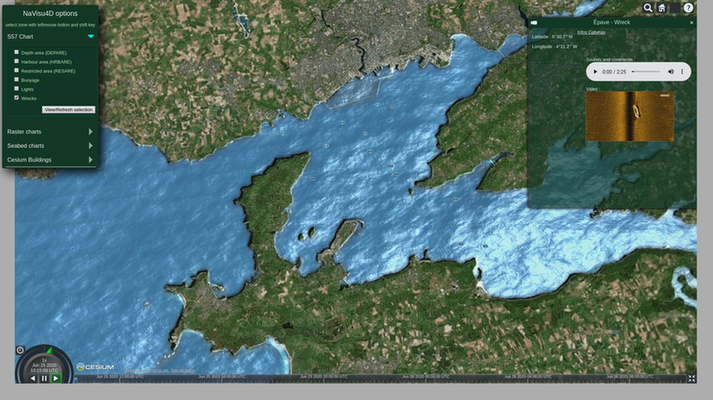
\includegraphics[width=15cm]{images/epaves/epave_1.png}
}
\begin{figure}[ht]
\caption{\label{equiProj}\textit{L'épave du Gobetas}}
\end{figure}
\end{center}
%%%%%%%%%%%%%%%%%%%%%%%%%%%%%%%%%%%%%%%%%%%%%%%%%%%%%%%%%%%%%%%%%%%%%%%
\newpage
%%%%%%%%%%%%%%%%%%%%%%%%%%%%%%%%%%%%%%%%%%%%%%%%%%%%%%%%%%%%%%%%%%%%%%%
\section{Les zones d'intérêt}
Toute donnée géoréférencée, sous format GeoTIFF, Shapefile, WMS, WMTS, GeoJSON, \ldots peut être représentée, exemples :
\subsection{Habitats terrestres et marins : EUNIS 
(European Nature Information System)}
%%%%%%%%%%%%%%%%%%%%%%%%%%%%%%%%%%%%%%%%%%%%%%%%%%%%%%%%%%%%%%%%%%%%%%%
\begin{center}
\framebox[1\width]{
	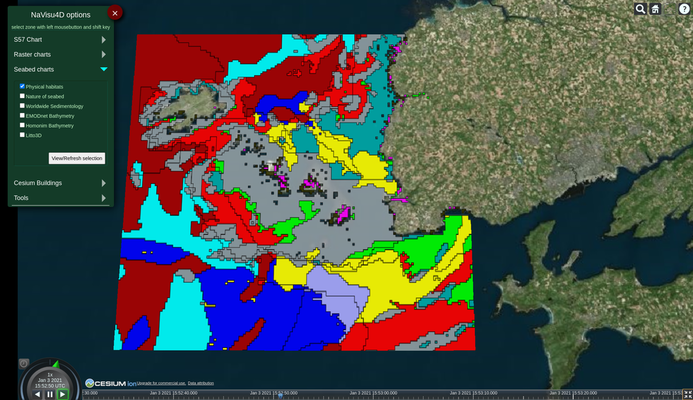
\includegraphics[width=15cm, height=7.5cm]{images/sedimento/habitatPhysique.png}
}
\begin{figure}[ht]
\caption{\label{sedimento0}\textit{Habitats physiques}}
\end{figure}
\end{center}
%%%%%%%%%%%%%%%%%%%%%%%%%%%%%%%%%%%%%%%%%%%%%%%%%%%%%%%%%%%%%%%%%%%%%%%
%%%%%%%%%%%%%%%%%%%%%%%%%%%%%%%%%%%%%%%%%%%%%%%%%%%%%%%%%%%%%%%%%%%%%%%
\begin{center}
\framebox[1\width]{
	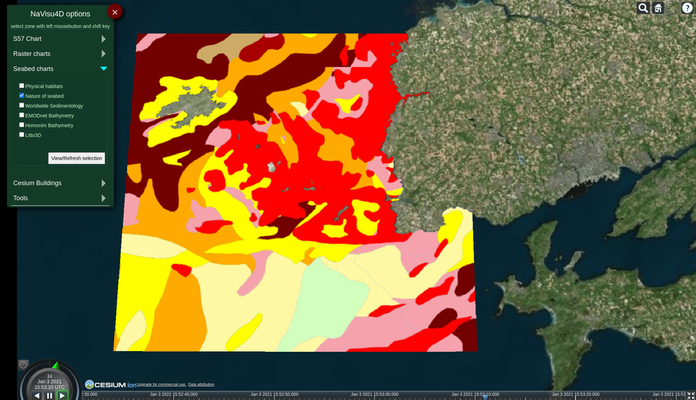
\includegraphics[width=15cm, height=7.5cm]{images/sedimento/natureDuFond.png}
}
\begin{figure}[ht]
\caption{\label{sedimento1}\textit{Nature du fond : Mer d'Iroise}}
\end{figure}
\end{center}
%%%%%%%%%%%%%%%%%%%%%%%%%%%%%%%%%%%%%%%%%%%%%%%%%%%%%%%%%%%%%%%%%%%%%%%
%%%%%%%%%%%%%%%%%%%%%%%%%%%%%%%%%%%%%%%%%%%%%%%%%%%%%%%%%%%%%%%%%%%%%%%
\begin{center}
\framebox[1\width]{
	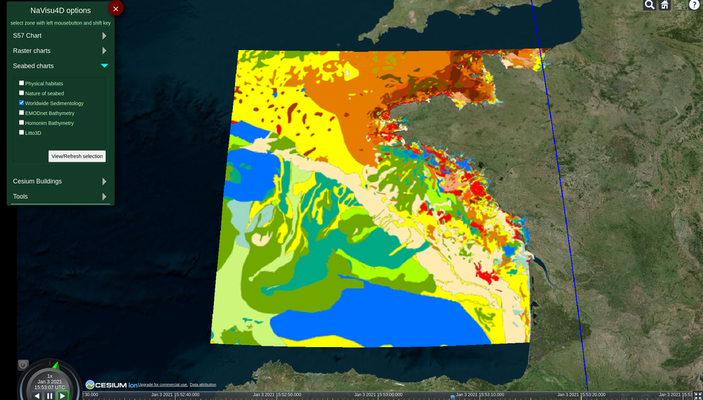
\includegraphics[width=15cm, height=7.5cm]{images/sedimento/wwSedimentologie.png}
}
\begin{figure}[ht]
\caption{\label{sedimento2}\textit{Nature du fond : couverture mondiale}}
\end{figure}
\end{center}
%%%%%%%%%%%%%%%%%%%%%%%%%%%%%%%%%%%%%%%%%%%%%%%%%%%%%%%%%%%%%%%%%%%%%%%
\chapter{Les objets 3D}
\section{Les bâtiments}
\subsection{OSM Building}
Il est possible d'afficher la couche OSM Building \href{https://osmbuildings.org/}{https://osmbuildings.org/} \\
c'est ainsi que 350 millions de bâtiments dans le monde sont visibles, la possibilité d'extraire leurs caractéristiques est en cours de développement.
%%%%%%%%%%%%%%%%%%%%%%%%%%%%%%%%%%%%%%%%%%%%%%%%%%%%%%%%%%%%%%%%%%%%%%%
\begin{center}
\framebox[1\width]{
	\includegraphics[width=15cm]{images/osmb/osmb_0.png}
}
\begin{figure}[ht]
\caption{\label{equiProj}\textit{Survol de la ville de Brest}}
\end{figure}
\end{center}
%%%%%%%%%%%%%%%%%%%%%%%%%%%%%%%%%%%%%%%%%%%%%%%%%%%%%%%%%%%%%%%%%%%%%%%
%%%%%%%%%%%%%%%%%%%%%%%%%%%%%%%%%%%%%%%%%%%%%%%%%%%%%%%%%%%%%%%%%%%%%%%
\begin{center}
\framebox[1\width]{
	\includegraphics[width=15cm]{images/osmb/osmb_1.png}
}
\begin{figure}[ht]
\caption{\label{equiProj}\textit{Brest : le port}}
\end{figure}
\end{center}
%%%%%%%%%%%%%%%%%%%%%%%%%%%%%%%%%%%%%%%%%%%%%%%%%%%%%%%%%%%%%%%%%%%%%%%
\subsection{CityGML}

CityGML \href{http://www.citygml.org/}{http://www.citygml.org/} est un format de données de l'OGC (Open Geospatial Consortium)
 \href{https://www.ogc.org/standards/citygml}{https://www.ogc.org/standards/citygml} pour la modélisation des villes. En particulier les villes connectées ou Smart Cities. Par exemple, la ville de Brest, met à la disposition du public l'ensemble des bâtiments au format CityGML, il est possible de les visualiser avec plus de détails que par OSM Building.
 %%%%%%%%%%%%%%%%%%%%%%%%%%%%%%%%%%%%%%%%%%%%%%%%%%%%%%%%%%%%%%%%%%%%%%%
\begin{center}
\framebox[1\width]{
	\includegraphics[width=15cm]{images/citygml/cityGML.png}
}
\begin{figure}[ht]
\caption{\label{equiProj}\textit{Brest : le port (SIG Brest Métropole)}}
\end{figure}
\end{center}
%%%%%%%%%%%%%%%%%%%%%%%%%%%%%%%%%%%%%%%%%%%%%%%%%%%%%%%%%%%%%%%%%%%%%%%
\section{Les objets statiques}
Il est possible, après mise au format glTF, d'intégrer des modèles 3D détaillés de bâtiments, d'ouvrage d'art, de navires, \ldots Ces objets sont aussi interrogeables et pour certains il peut y avoir des modifications dynamiques, position, attitude, apparence, \ldots
%%%%%%%%%%%%%%%%%%%%%%%%%%%%%%%%%%%%%%%%%%%%%%%%%%%%%%%%%%%%%%%%%%%%%%%
\begin{center}
\framebox[1\width]{
	\includegraphics[width=14cm]{images/models/models_0.png}
}
\begin{figure}[ht]
\caption{\label{equiProj}\textit{Le phare du Portzic}}
\end{figure}
\end{center}
%%%%%%%%%%%%%%%%%%%%%%%%%%%%%%%%%%%%%%%%%%%%%%%%%%%%%%%%%%%%%%%%%%%%%%%
%%%%%%%%%%%%%%%%%%%%%%%%%%%%%%%%%%%%%%%%%%%%%%%%%%%%%%%%%%%%%%%%%%%%%%%
\begin{center}
\framebox[1\width]{
	\includegraphics[width=14cm]{images/models/models_1.png}
}
\begin{figure}[ht]
\caption{\label{equiProj}\textit{Le phare du Créach}}
\end{figure}
\end{center}
%%%%%%%%%%%%%%%%%%%%%%%%%%%%%%%%%%%%%%%%%%%%%%%%%%%%%%%%%%%%%%%%%%%%%%%
%%%%%%%%%%%%%%%%%%%%%%%%%%%%%%%%%%%%%%%%%%%%%%%%%%%%%%%%%%%%%%%%%%%%%%%
\begin{center}
\framebox[1\width]{
	\includegraphics[width=14cm]{images/models/razDeSein.png}
}
\begin{figure}[ht]
\caption{\label{equiProj}\textit{Le Raz de sein (réel)}}
\end{figure}
\end{center}
%%%%%%%%%%%%%%%%%%%%%%%%%%%%%%%%%%%%%%%%%%%%%%%%%%%%%%%%%%%%%%%%%%%%%%%
%%%%%%%%%%%%%%%%%%%%%%%%%%%%%%%%%%%%%%%%%%%%%%%%%%%%%%%%%%%%%%%%%%%%%%%
\begin{center}
\framebox[1\width]{
	\includegraphics[width=14cm]{images/models/razDeSeinVirtuel.png}
}
\begin{figure}[ht]
\caption{\label{equiProj}\textit{Le Raz de sein (virtuel)}}
\end{figure}
\end{center}
\section{Les objets dynamiques}
Les modèles 3D peuvent être animés
%%%%%%%%%%%%%%%%%%%%%%%%%%%%%%%%%%%%%%%%%%%%%%%%%%%%%%%%%%%%%%%%%%%%%%%
\begin{center}
\framebox[1\width]{
	\includegraphics[width=14cm]{images/dynamique/dyna_0.png}
}
\begin{figure}[ht]
\caption{\label{anim0}\textit{Avions, navires,\ldots}}
\end{figure}
\end{center}
%%%%%%%%%%%%%%%%%%%%%%%%%%%%%%%%%%%%%%%%%%%%%%%%%%%%%%%%%%%%%%%%%%%%%%%
Des parties de modèles peuvent aussi être animées
%%%%%%%%%%%%%%%%%%%%%%%%%%%%%%%%%%%%%%%%%%%%%%%%%%%%%%%%%%%%%%%%%%%%%%%
\begin{center}
\framebox[1\width]{
	\includegraphics[width=14cm]{images/dynamique/grueBrestPrepa.png}
}
\begin{figure}[ht]
\caption{\label{anim1}\textit{Préparation du mouvement d'un composant en gltf}}
\end{figure}
\end{center}
%%%%%%%%%%%%%%%%%%%%%%%%%%%%%%%%%%%%%%%%%%%%%%%%%%%%%%%%%%%%%%%%%%%%%%%
%%%%%%%%%%%%%%%%%%%%%%%%%%%%%%%%%%%%%%%%%%%%%%%%%%%%%%%%%%%%%%%%%%%%%%%
\begin{center}
\framebox[1\width]{
	\includegraphics[width=14cm]{images/dynamique/grues_2.png}
}
\begin{figure}[ht]
\caption{\label{anim2}\textit{Les grues, mobiles,  sur le port de commerce de Brest}}
\end{figure}
\end{center}
%%%%%%%%%%%%%%%%%%%%%%%%%%%%%%%%%%%%%%%%%%%%%%%%%%%%%%%%%%%%%%%%%%%%%%%

\chapter{Le monde sous-marin}
Définir une zone rectangulaire  nous permet de plonger sous la mer, d'y placer des structures, des modèles de terrains bathymétriques et d'observer depuis le fond.
%%%%%%%%%%%%%%%%%%%%%%%%%%%%%%%%%%%%%%%%%%%%%%%%%%%%%%%%%%%%%%%%%%%%%%%
\begin{center}
\framebox[1\width]{
	\includegraphics[width=14cm]{images/underground/underground_0.png}
}
\begin{figure}[ht]
\caption{\label{equiProj}\textit{Sélection de la zone}}
\end{figure}
\end{center}
%%%%%%%%%%%%%%%%%%%%%%%%%%%%%%%%%%%%%%%%%%%%%%%%%%%%%%%%%%%%%%%%%%%%%%%
%%%%%%%%%%%%%%%%%%%%%%%%%%%%%%%%%%%%%%%%%%%%%%%%%%%%%%%%%%%%%%%%%%%%%%%
\begin{center}
\framebox[1\width]{
	\includegraphics[width=14cm]{images/underground/underground_1.png}
}
\begin{figure}[ht]
\caption{\label{equiProj}\textit{Le Gobetas (flottant !)}}
\end{figure}
\end{center}
%%%%%%%%%%%%%%%%%%%%%%%%%%%%%%%%%%%%%%%%%%%%%%%%%%%%%%%%%%%%%%%%%%%%%%%
%%%%%%%%%%%%%%%%%%%%%%%%%%%%%%%%%%%%%%%%%%%%%%%%%%%%%%%%%%%%%%%%%%%%%%%
\begin{center}
\framebox[1\width]{
	\includegraphics[width=14cm, height=8cm]{images/underground/underground_2.png}
}
\begin{figure}[ht]
\caption{\label{equiProj}\textit{Le Gobetas, vu depuis le fond}}
\end{figure}
\end{center}
%%%%%%%%%%%%%%%%%%%%%%%%%%%%%%%%%%%%%%%%%%%%%%%%%%%%%%%%%%%%%%%%%%%%%%%
\chapter{La vidéo}
%%%%%%%%%%%%%%%%%%%%%%%%%%%%%%%%%%%%%%%%%%%%%%%%%%%%%%%%%%%%%%%%%%%%%%%
\section{La vidéo dans l'univers 3D}
\begin{itemize}
\item A chaque point remarquable, il est possible d'associer des données textuelles, des images ou des vidéos,
dans le panneau d'information.
\item Les vidéos peuvent être appelées depuis des points remarquables pour être projetées sur des surfaces 3D.
\end{itemize}
\begin{center}
\framebox[1\width]{
	\includegraphics[width=14cm, height=8cm]{images/video/video_0.png}
}
\begin{figure}[ht]
\caption{\label{equiProj}\textit{la Vidéo 3D}}
\end{figure}
\end{center}
%%%%%%%%%%%%%%%%%%%%%%%%%%%%%%%%%%%%%%%%%%%%%%%%%%%%%%%%%%%%%%%%%%%%%%%
\newpage
\section{Les webcams}
Par ailleurs des données venant de webcams positionnées sur le territoire, peuvent être visualisées sur un simple clic
sur le site, un phare, un amer, \ldots
%%%%%%%%%%%%%%%%%%%%%%%%%%%%%%%%%%%%%%%%%%%%%%%%%%%%%%%%%%%%%%%%%%%%%%%
\begin{center}
\framebox[1\width]{
	\includegraphics[width=14cm, height=8cm]{images/video/webcam_0.png}
}
\begin{figure}[ht]
\caption{\label{equiProj}\textit{Sélection des Webcams}}
\end{figure}
\end{center}
%%%%%%%%%%%%%%%%%%%%%%%%%%%%%%%%%%%%%%%%%%%%%%%%%%%%%%%%%%%%%%%%%%%%%%%
%%%%%%%%%%%%%%%%%%%%%%%%%%%%%%%%%%%%%%%%%%%%%%%%%%%%%%%%%%%%%%%%%%%%%%%
\begin{center}
\framebox[1\width]{
	\includegraphics[width=14cm, height=8cm]{images/video/pipInfoBox.png}
}
\begin{figure}[ht]
\caption{\label{equiProj}\textit{La webcam de l'Ile de Sein}}
\end{figure}
\end{center}
%%%%%%%%%%%%%%%%%%%%%%%%%%%%%%%%%%%%%%%%%%%%%%%%%%%%%%%%%%%%%%%%%%%%%%%
\chapter{Les entrées/sorties}
Pour connecter \nav aux capteurs d'un mobile (navire, aéronef), nous avons fait le choix d'utiliser SignalK.
\section{SignalK}
SignalK  \href{http://signalk.org/}{http://signalk.org/} est une application client/serveur qui peut être installée sur un poste, un bateau par exemple. Le rôle du serveur est de faire l'acquisition  des données  client : position GPS, AIS, données moteur \ldots De les multiplexer, de les formater et de les diffuser. \nav va ensuite interroger ce serveur pour la visualisation.
%%%%%%%%%%%%%%%%%%%%%%%%%%%%%%%%%%%%%%%%%%%%%%%%%%%%%%%%%%%%%%%%%%%%%%%
\begin{center}
\framebox[1\width]{
	\includegraphics[width=12cm]{images/signalK/signalK_0.png}
}
\begin{figure}[ht]
\caption{\label{sinoptique}\textit{Sinoptique de SignalK}}
\end{figure}
\end{center}
%%%%%%%%%%%%%%%%%%%%%%%%%%%%%%%%%%%%%%%%%%%%%%%%%%%%%%%%%%%%%%%%%%%%%%%
SignalK est une application complètement indépendante de \nav, il appartient à l'utilisateur voulant
s'en servir de l'installer sur sa propre machine.
SignalK fonctionne sur différentes plateformes, par exemple sur Raspberry : \\
 \href{https://github.com/SignalK/signalk-server/blob/master/raspberry\_pi\_installation.md}{
 https://github.com/SignalK/signalk-server/blob/master/raspberry\_pi\_installation.md} \\
 Par contre sur RaspBerry, \nav nécessite un RPI4. Le serveur \nav peut être évidement sur une machine différente de celle de visualisation.
\section{Initialisation SignalK}
Voir documentation spécifique  : \href{http://signalk.org/specification/1.5.0/doc/}{http://signalk.org/specification/1.5.0/doc/}
\subsection{Choix des données en entrée}
\subsubsection{Data type}
\begin{itemize}
\item NMEA 2000
\item NMEA 0183
\item SignalK
\item Seatalk (GPIO)
\item File Stream
\end{itemize}
\subsubsection{Data source}
Exemple pour des données de type NMEA 0183
\begin{itemize}
\item Serial
\item TCP Client
\item TCP server
\item UDP
\item GPSD
\end{itemize}
%%%%%%%%%%%%%%%%%%%%%%%%%%%%%%%%%%%%%%%%%%%%%%%%%%%%%%%%%%%%%%%%%%%%%%%
\begin{center}
\framebox[1\width]{
	\includegraphics[width=14cm]{images/signalK/dataConnection.png}
}
\begin{figure}[ht]
\caption{\label{data}\textit{Choix des données en entrée}}
\end{figure}
\end{center}
%%%%%%%%%%%%%%%%%%%%%%%%%%%%%%%%%%%%%%%%%%%%%%%%%%%%%%%%%%%%%%%%%%%%%%%
\subsection{Visualisation des données}
%%%%%%%%%%%%%%%%%%%%%%%%%%%%%%%%%%%%%%%%%%%%%%%%%%%%%%%%%%%%%%%%%%%%%%%
\begin{center}
\framebox[1\width]{
	\includegraphics[width=13cm]{images/signalK/skPanel.png}
}
\begin{figure}[ht]
\caption{\label{data}\textit{Panneau des instruments (extrait) des données du fichier Route.nmea}}
\end{figure}
\end{center}
%%%%%%%%%%%%%%%%%%%%%%%%%%%%%%%%%%%%%%%%%%%%%%%%%%%%%%%%%%%%%%%%%%%%%%%
\section{Simulations : rejeu de fichiers de points GNSS (expérimental)}
Les données en entrée sont des fichiers au format : NMEA183, N2K, \ldots
Deux cas de rejeu sont possible.
Dans les deux cas, les informations sont interprétées par SignalK, transformées en un format JSON,  puis interprétées par \nav. SignalK doit être configuré pour lire le fichier de rejeu.
\begin{itemize}
\item Simulation statique : les différents points de données sont affichés.
\item Simulation dynamique : en plus de l'affichage des points, un mobile est représenté parcourant les tracks. La vitesse de déplacement est ajustable, elle peut aussi être inversée.
\end{itemize}
Procédure : 
\begin{enumerate}
\item Coté SignalK après connexion par ex: {\tt localhost:3000}
\begin{enumerate}
\item Server
\item Data connections
\item Sélectionner le type File Stream
\item Indiquer le nom du fichier à lire
\end{enumerate}
\item Coté NaVisu4D
\begin{enumerate}
\item Item Communication
\item Item SignalK Connection
\item Item Trail (option)
\item Bouton Connect/Disconnect
\end{enumerate}
\end{enumerate}


%%%%%%%%%%%%%%%%%%%%%%%%%%%%%%%%%%%%%%%%%%%%%%%%%%%%%%%%%%%%%%%%%%%%%%%
\begin{center}
\framebox[1\width]{
	\includegraphics[width=14cm]{images/signalK/signalK_1.png}
}
\begin{figure}[ht]
\caption{\label{equiProj}\textit{De Morgat à La Baie de Lampaul (Ouessant)}}
\end{figure}
\end{center}
%%%%%%%%%%%%%%%%%%%%%%%%%%%%%%%%%%%%%%%%%%%%%%%%%%%%%%%%%%%%%%%%%%%%%%%
%%%%%%%%%%%%%%%%%%%%%%%%%%%%%%%%%%%%%%%%%%%%%%%%%%%%%%%%%%%%%%%%%%%%%%%
\begin{center}
\framebox[1\width]{
	\includegraphics[width=14cm]{images/signalK/signalK_2.png}
}
\begin{figure}[ht]
\caption{\label{equiProj}\textit{Simulation GNSS, suivi caméra}}
\end{figure}
\end{center}
%%%%%%%%%%%%%%%%%%%%%%%%%%%%%%%%%%%%%%%%%%%%%%%%%%%%%%%%%%%%%%%%%%%%%%%
\newpage
\section{Visualisation "temps réel" (expérimental)}
A présent les données viennent des capteurs du navire, via SignalK. Le flux de données est traité de manière 
asynchrone. Le temps de mise en forme des données et ensuite d'affichage peut ne pas permettre le traitement de
toute les données. Celles-ci seront perdues, pour assurer un rendu fluide du mobile.\\
Procédure : 
\begin{enumerate}
\item Coté SignalK après connexion par ex: {\tt localhost:3000}
\begin{enumerate}
\item Server
\item Data connections
\item Sélectionner le type : NMEA 2000, NMEA183, \ldots
\item Indiquer la source : Serial, UDP, TCP, \ldots
\end{enumerate}
\item Coté NaVisu4D
\begin{enumerate}
\item Item Communication
\item Item SignalK Connection
\item Item Trail (option)
\item Bouton Connect/Disconnect
\end{enumerate}
\end{enumerate}
%%%%%%%%%%%%%%%%%%%%%%%%%%%%%%%%%%%%%%%%%%%%%%%%%%%%%%%%%%%%%%%%%%%%%%%
\chapter{L'API REST}
Ce chapitre sera utile aux développeurs voulant associer \nav à une autre application. Il sera alors possible de complètement piloter NaVisu4D depuis cette ou ces applications à travers Internet, grâce à l'interface API REST
et de partager ce comportement entre plusieurs clients \nav.
L'idée est la suivante : partant d'une simple URL, comment soit piloter, soit récupérer des informations depuis \nav ? L'API REST fonctionne un peu comme le CRUD des bases de données, pour aller vite, on a à notre disposition les méthodes :
GET, POST, PUT, DELETE,\ldots\\
\href{https://fr.wikipedia.org/wiki/Representational\_state\_transfer}{https://fr.wikipedia.org/wikiRepresentational\_state\_transfer}\\
\begin{itemize}
\item GET permet de récupérer des données
\item POST de rajouter des entités à une ressource
\item PUT  modifie les données
\item DELETE peut en supprimer
\end{itemize}


Par exemple l'association SMAUG, à partir d'une maquette physique, d'une zone géographique, capture à l'aide d'une caméra le déplacement d'un curseur, un petit bateau. Après traitement cet objet est localisé géographiquement, régulièrement ces données sont alors transmises à l'univers virtuel \nav. faisant ainsi le lien entre les deux univers : une maquette physique et un espace virtuel.

Cette API peut fonctionner en local avec une ou plusieurs applications \nav, mais aussi à travers le web. Un serveur associé au site {\tt http://www.terrevirtuelle.org}  peut alors donner accès au partage d'applications \nav à différents clients.
%%%%%%%%%%%%%%%%%%%%%%%%%%%%%%%%%%%%%%%%%%%%%%%%%%%%%%%%%%%%%%%%%%%%%%%
\begin{center}
\framebox[1\width]{
	\includegraphics[width=14cm]{images/smaug/smaug.png}
}
\begin{figure}[ht]
\caption{\label{smaug0}\textit{La maquette SMAUG}}
\end{figure}
\end{center}
%%%%%%%%%%%%%%%%%%%%%%%%%%%%%%%%%%%%%%%%%%%%%%%%%%%%%%%%%%%%%%%%%%%%%%%
\begin{center}
\framebox[1\width]{
	\includegraphics[width=14cm]{images/smaug/benchyYellow.png}
}
\begin{figure}[ht]
\caption{\label{smaug}\textit{Visualisation du curseur SMAUG dans \nav}}
\end{figure}
\end{center}
%%%%%%%%%%%%%%%%%%%%%%%%%%%%%%%%%%%%%%%%%%%%%%%%%%%%%%%%%%%%%%%%%%%%%%%
\newpage
\section{Principes de la modification de l'état d'un objet}

Si on veut par exemple asservir la caméra de \nav à une consigne de type \{latitude, longitude, altitude\},
on choisit la méthode PUT :
{\small
\begin{verbatim}
curl -X PUT "http://localhost:3000/control?cmd=position&origin=SMAUG&target=camera
&latitude=48.00&longitude=-4.50&altitude=30000&heading=180.0&pitch=0.0&roll=10.0"
\end{verbatim}
}

Structure de la requête :
\begin{enumerate}
\item instruction :  {\tt curl -X PUT }
\item URL : {\tt http://localhost:3000/}
\item route : {\tt control}
\item commande : {\tt position, flyTo}
\item origine : nom du client par exemple : {\tt SMAUG}
\item cible : {\tt camera}
\item paramètres : {\tt latitude=48.00, longitude=-4.50, altitude=30000, heading=180.0, \\
pitch=0.0, roll=10.0"}
\end{enumerate}

Cette requête est envoyée au serveur REST, pour être mise en forme, puis envoyée à \nav via une WebSocket, où elle est interprétée. Résultat la caméra est déplacée. Dans cet exemple, le serveur APIRest est local, il peut être nimporte où sur le réseau.

La commande {\tt position} permet d'aller à cette position immédiatement, la commande {\tt flyTo} permet de se déplacer vers cette position.\\

Dans l'exemple précédent \nav reçoit :

\begin{verbatim}{"cmd":"position","origin":"SMAUG","target":"camera",
"latitude":"48.00","longitude":"-4.50","altitude":"30000",
"heading":"180.0","pitch":"0.0","roll":"10.0"}
\end{verbatim}
ou
\begin{verbatim}{"cmd":"flyTo","origin":"SMAUG","target":"camera",
"latitude":"48.00","longitude":"-4.50","altitude":"30000",
"heading":"180.0","pitch":"0.0","roll":"10.0"}
\end{verbatim}

\section{Recherche d'informations}
On pourra aussi utiliser GET, pour obtenir toutes les informations sur l'application et aussi la connexion à nos bases de données via GeoServer ou encore les WebServices auxquels \nav est connectée. ({\em à compléter})
\newpage

\section{Exemple de connexion sur le web}
\begin{enumerate}
\item Lancer \nav : \href{http://www.terrevirtuelle.org/Navisu4D/}{http://www.terrevirtuelle.org/Navisu4D/}
\item Connecter \nav au serveur APIRest : Menu de gauche : {\tt Tools/Rest API Server}
%%%%%%%%%%%%%%%%%%%%%%%%%%%%%%%%%%%%%%%%%%%%%%%%%%%%%%%%%%%%%%%%%%%%%%%
\begin{center}
\framebox[1\width]{
	\includegraphics[width=14cm]{images/apiRest/apiRest.png}
}
\begin{figure}[ht]
\caption{\label{apiRest}\textit{Connexion au serveur}}
\end{figure}
\end{center}
%%%%%%%%%%%%%%%%%%%%%%%%%%%%%%%%%%%%%%%%%%%%%%%%%%%%%%%%%%%%%%%%%%%%%%%
\item A partir d'une console ou d'une application, préparer et envoyer la requête au serveur (\textcolor{red}{l'adresse est à demander aux administrateurs \nav})
\end{enumerate}

\section{Exemple d'envoi de la requête en Python}

\begin{Verbatim}[commandchars=\\\{\}]
import requests
requests.put('http:\textcolor{red}{adresse\_du\_serveur:port}/control?cmd=position&origin=SMAUG
&target=camera
&latitude=48.00&longitude=-4.50&altitude=30000
&heading=180.0&pitch=0.0&roll=10.0')
\end{Verbatim}

Selon votre configuration, cet exemple réclame, peut être, l'installation du module {\tt request}
\begin{verbatim}
$ pip install requests
\end{verbatim}
Evidemment il est possible  de tout faire en local. Il suffit d'installer le serveur :\\
 \textcolor{blue}{\href{https://github.com/terre-virtuelle/ApiRestNaVisu4D}{https://github.com/terre-virtuelle/ApiRestNaVisu4D}}
 


\chapter*{Fin}
%%%%%%%%%%%%%%%%%%%%%%%%%%%%%%%%%%%%%%%%%%%%%%%%%%%%%%%%%%%%%%%%%%%%%%%
\begin{center}
\framebox[1\width]{
	\includegraphics[width=14cm]{images/fin/leMinou.png}
}
\begin{figure}[ht]
\caption{\label{equiProj}\textit{Coucher de soleil sur le phare du Minou}}
\end{figure}
\end{center}
%%%%%%%%%%%%%%%%%%%%%%%%%%%%%%%%%%%%%%%%%%%%%%%%%%%%%%%%%%%%%%%%%%%%%%%
\subsection*{Contacts}
courriel : {\tt sergemorvan29@gmail.com}\\
\hbox{}\hspace{0.6cm}courriel : {\tt dom.marques@terrevirtuelle.org}\\
 \hbox{}\hspace{6cm}\href{http://www.terrevirtuelle.org/}{http://www.terrevirtuelle.org/}



	 \tableofcontents
	\label{fin}
	
	% ------------------------------------------------------------------------------
\end{document}
